\documentclass[titlepage, 11pt]{article}
\usepackage[fntef]{ctexcap}
\usepackage{txfonts}
\usepackage{hyperref}
\usepackage{fancyhdr}
\usepackage{geometry}
\usepackage{graphicx}
\usepackage{multirow}
\usepackage{booktabs}
\usepackage{enumerate}
\usepackage{txfonts}
\usepackage{clrscode3e}
\usepackage{float}
\usepackage{caption}
\usepackage{subfigure}
\usepackage{hyperref}
\usepackage{fontspec}
%\usepackage{fontspec-xetex}
\CTEXsetup[name={第,节},number={\chinese{section}}]{section}
\CTEXsetup[number={\chinese{subsection}}]{subsection}
\setmainfont{Times New Roman}
\geometry{bottom=2.5cm,top=3.5cm,left=2.5cm,right=2.5cm}
\pagestyle{fancy}
%\hyperref{colorlinks,linkcolor=red, anchorcolor=blue, citecolor=green}
\begin{document}
	\title{\vspace{-25mm}数字逻辑电路实验报告\\\vspace{15mm}\Huge\textbf{第十三次实验:简易计算机系统}\vspace{60mm}}
	\author{张铭方\\161220169\\16级计算机系5班\\\texttt{161220169@smail.nju.edu.cn}\and 许致明\\161180162\\16级计算机系5班\\\texttt{161180162@smail.nju.edu.cn}}\date{\vspace{30mm}\today}
	\maketitle
	\section{实验目的}
	本实验的目标是在Nexys 4开发板上实现一个简易的计算机系统,能够运行简单的指令,包括循环、整数计算、函数调用、递归等。这些指令使用RISC方式编写,存储在开发板的存储器(ROM)中。开发板的另一部分存储器(RAM)用来保存程序运行中所需的数据。此外,在完成后,开发板还具有一定的输出功能,程序输入通过向ROM中初始化相应的机器码实现。
	\section{实验原理}
	\subsection{计算机系统简介}
	计算机系统主要由CPU和外部设备组成。CPU是系统中最重要的部分,它负责控制系统运行和信息处理。外部设备负责和外界进行交互,使得计算机的可以接受输入,产生相应的输出。本实验需要实现一个简化的计算机系统。下面对两种基本的系统结构做简要介绍。\par 
	%\begin{enumerate}	
	%\end{enumerate}
	第一种是冯·诺伊曼结构,这种结构被现代的大多数CPU所使用。在这种结构下,处理器使用同一个存储器,经过同一个总线传输,具有以下特点:
	\begin{enumerate}
		\item 结构上由运算器、控制器、存储器和输入/输出设备组成;
		\item 存储器是按地址访问的,每个地址是唯一的;
		\item 指令和数据都是以二进制形式存储的;
		\item 指令按顺序执行,即一般指令按照存储顺序执行,程序的分支、循环由转移指令实现;
		\item 以运算器为中心,在输入输出设备与控制器之间的数据传送都途径运算器。运算器、存储器、输入输出设备的操作以及它们之间的联系都由控制器集中控制。
	\end{enumerate}\par 
	%\end{enumerate}
	第二种是哈佛结构,它使用两个独立的存储模块,分别存储指令和数据,并具有一条独立的地址总线和一条独立的数据总线,具有以下特点:
	\begin{enumerate}
		\item 每个存储块都不允许指令和数据并存,以便实现并行处理;
		\item 利用公共地址总线访问两个存储模块(程序存储模块ROM和输出存储模块RAM),公用数据总线则被用来完成程序存储模块或数据存储模块与CPU之间的数据传输;
		\item 地址总线和数据总线由程序存储器和数据存储器分时共用。
	\end{enumerate}\par 
	数字信号处理一般需要较大的运算量和较高的运算速度,为了提高数据吞吐量,在数字信号处理中大多采用哈佛结构。本实验所构建的计算机系统就采用了哈佛结构。
	\subsection{RISC架构简介}
	\subsubsection{RISC架构的基本特征}
	RISC,即Reduced Instruction Set Computer,是精简指令集计算机的简称,与它相对的是CISC(Complex Instruction Set Computer)。RISC架构主要具有以下特点:
	\begin{enumerate}
	\item 只包含一些使用频率较高的指令,并用这些指令的组合来实现较为复杂指令的功能;
	\item 指令长度固定,指令格式、寻址方式比CICS少;
	\item 只有加载、存储两条指令需要访问内存,其他指令都是在寄存器和寄存器或寄存器和立即数之间进行操作;
	\item CPU中包含多个通用寄存器,执行指令过程中的数据均暂存在寄存器中,提高指令的执行速度;
	\item 常常采用流水线技术,这样大部分指令可以在一个时钟周期内完成。还可以采用超标量和超流水线技术,使指令平均执行时间小于一个时钟周期;
	\item 控制器采用组合逻辑的控制方式,不使用微程序控制的方式。
	\end{enumerate}\par 
	CPU是计算机中的核心部件。RISC架构中的CPU进行信息处理时,主要进行如下两个步骤:
	\begin{enumerate}
		\item 将数据和指令(二进制串)读入到计算机的存储器中;
		\item 从第一条开始,按顺序执行程序,直至停机,结束运行。
	\end{enumerate}
	这一过程还可以用伪代码表示如下:
	\begin{codebox}
		\zi\proc{CPU-Execute}
		\li\While\const{true}
		\Do\li\proc{Fetch} instruction $Instr[PC]$
		\li \proc{Decode}  $Instr[PC]$
		\li\proc{Execute} $Instr[PC]$
		\li $PC\gets PC+1$
	\end{codebox}\par 
	为了实现这些操作,CPU至少需要具有以下功能:
	\begin{enumerate}
		\item 取指令:当程序已经在存储器(ROM)时,首先根据程序入口地址取出一条指令。需要CPU能发出正确的地址信息和产生控制读取存储器的信号;
		\item 指令译码:这一操作即需要分析出此二进制串的意义,获得
		它指示的操作内容,并且产生相应的操作控制命令;		
		\item 执行指令:根据指令译码得到的结果,产生相应的操作控制信号序列,控制运算器、存储器、输入输出设备的动作,完成这条指令的功能。其中包含对运算结果的处理(如设置标志位)以及下一条指令的地址的形成(如根据跳转指令更改PC的值)。
	\end{enumerate}\par 
	总而言之,CPU做为计算机系统的核心,主要的任务就是取出指令,解释指令,然后根据得到的结果执行相应的指令。在这些过程中,可能涉及到存储器(例如内存、内部寄存器)的读取、写入,PC内容更改(自增1或按条件跳转),以及和外部设备的数据交换(接收外设传来的输入信号,将输出信号发送给外设)。同时,CPU也需要产生相应的控制信号,使得其他部件能正确的工作。
	\subsubsection{RISC架构下CPU的基本构成}
	RISC CPU主要包括三方面的功能:数据存储、数据运算、时序控制。与此对应的就是三方面的硬件设备:寄存器和内存、运算器ALU、控制器。其基本结构如下面的图1所示:
	\begin{figure}[htb]
		\centering
		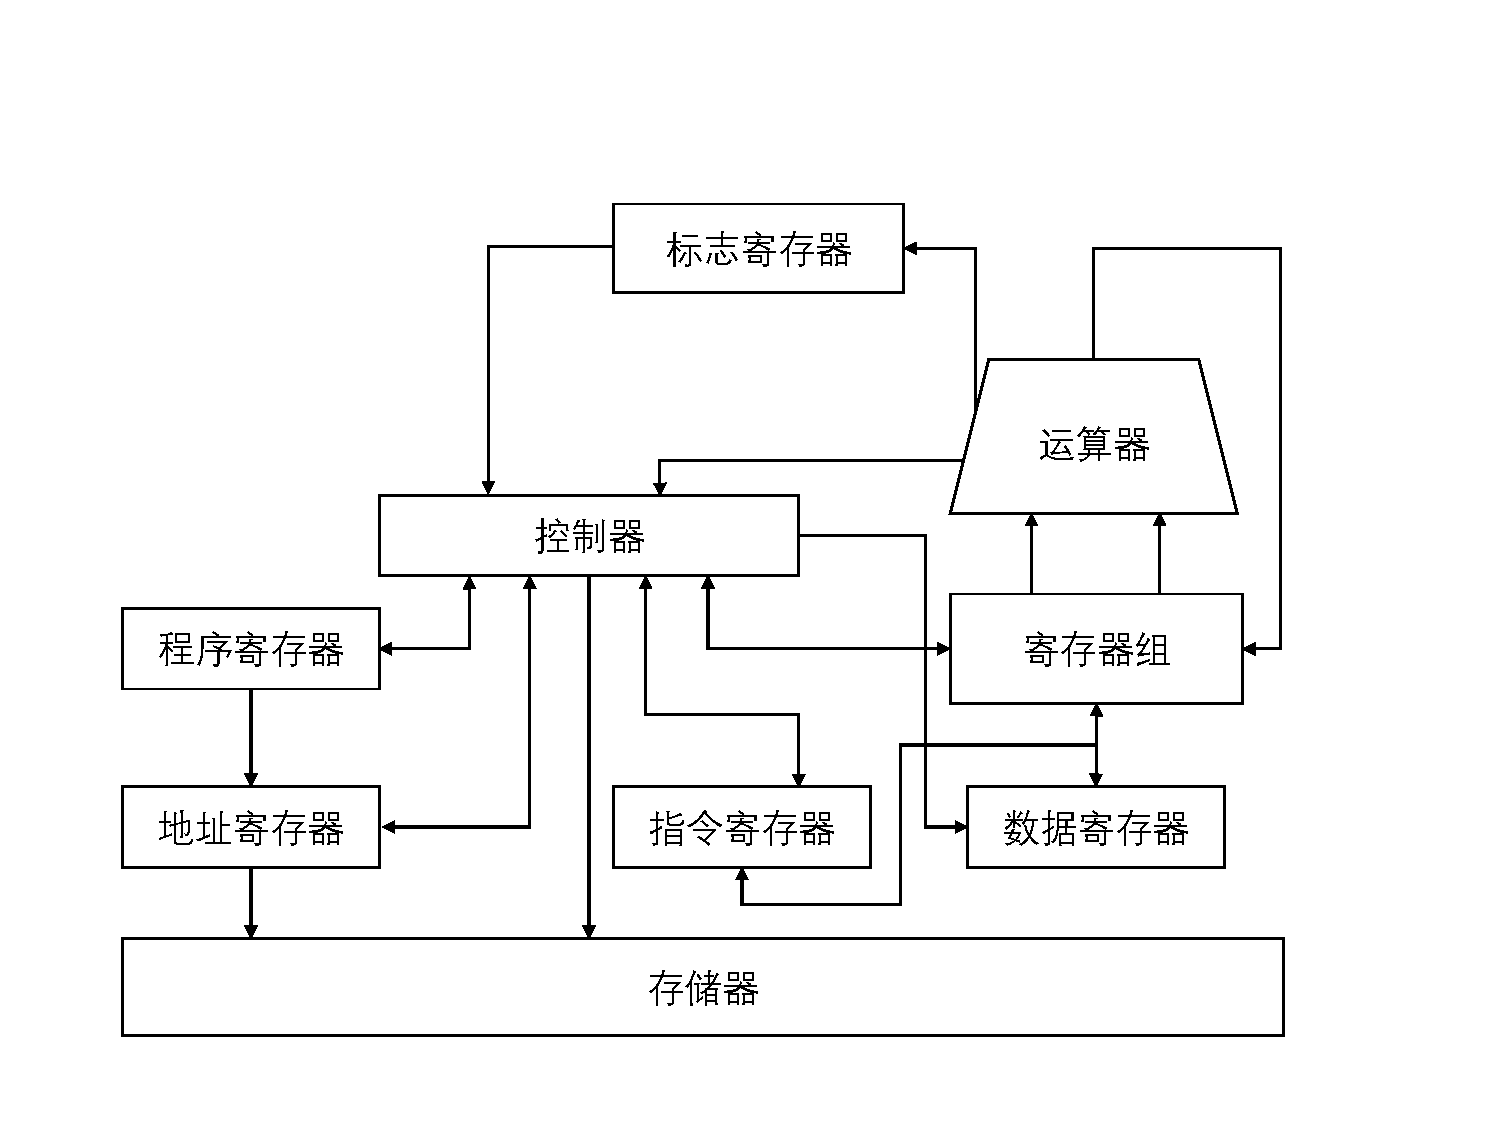
\includegraphics[scale=0.6]{1.pdf}
		\caption{RISC架构CPU的基本结构}
	\end{figure}\par 
	寄存器用于存放指令和数据,在此CPU设计中,包含了较多寄存器,这符合RISC架构的主要思想,即将指令执行过程中的各种数据存入到不同的寄存器中,减少访问速度较慢的内存的次数,从而提高处理器的运行速度。图中的箭头指明了数据在这条通路上的传输方向。通过多条通路,指令和数据能够独立传输、互不干扰,这样也能提高CPU的运行速度。
	\subsection{CPU的指令系统设计}
	在此次实验中,我们完成了一个16位的RISC架构指令集,共包含32条5个二进制位的定长指令,具有算术运算、存储读写、输入输出和逻辑控制这些基本功能。具体如表1所示:
	% Please add the following required packages to your document preamble:
	% \usepackage{multirow}
	\begin{table}[H]
		\centering
		\footnotesize
		\caption{指令系统概要}
		\label{my-label}
		\begin{tabular}{c|c|c|c}
			汇编指令格式            & 操作数   & 功能描述                                                           & 类型                     \\ \hline
			ADC \%SR, \%DR    & 00000 & R{[}DR{]}+R{[}SR{]}+CF→R{[}DR{]}                               & \multirow{14}{*}{算数逻辑} \\ \cline{1-3}
			SBB \%SR, \%DR    & 00001 & R{[}DR{]}-R{[}SR{]}-CF→R{[}DR{]}                               &                        \\ \cline{1-3}
			MUL \%SR, \%DR    & 00010 & R{[}DR{]}*R{[}SR{]}→R{[}DR{]}                                  &                        \\ \cline{1-3}
			DIV \%SR, \%DR    & 00011 & R{[}DR{]}/D{[}SR{]}→D{[}DR{]}(无符号)                             &                        \\ \cline{1-3}
			ADDI \$IMM, \%DR  & 00100 & R{[}DR{]}+\$IMM→R{[}DR{]}(寄存器与立即数相加)                           &                        \\ \cline{1-3}
			CMP \%SR, \%DR    & 00101 & R{[}DR{]}-R{[}SR{]}(只改变标志寄存器,若相等,则ZF=1)                        &                        \\ \cline{1-3}
			AND \%SR, \%DR    & 00110 & R{[}DR{]}\&R{[}SR{]}→R{[}DR{]}(按位与)                            &                        \\ \cline{1-3}
			OR \%SR, \%DR     & 00111 & R{[}DR{]}|R{[}SR{]}→R{[}DR{]}(按位或)                             &                        \\ \cline{1-3}
			NOT \%DR          & 01000 & $\sim$R{[}DR{]}→R{[}DR{]}(按位取反)                                &                        \\ \cline{1-3}
			XOR \%SR, \%DR    & 01001 & R{[}DR{]}\textasciicircum R{[}SR{]}→R{[}DR{]}(按位异或)            &                        \\ \cline{1-3}
			TEST \%SR, \%DR   & 01010 & R{[}DR{]}\textasciicircum R{[}SR{]}(根据结果改变标志寄存器ZF)             &                        \\ \cline{1-3}
			SHL \%DR          & 01011 & R{[}DR{]}$<<$1→R{[}DR{]}(逻辑或算数左移,最高位入CF)         &                        \\ \cline{1-3}
			SHR \%DR          & 01100 & R{[}DR{]}$>>$1→R{[}DR{]}(逻辑右移,高位补0,最低位入CF) &                        \\ \cline{1-3}
			SAR \%DR          & 01101 & R{[}DR{]}$>>$1→R{[}DR{]}(算术右移,高位补符)        &                        \\ \hline
			IN PORT, \%DR     & 01110 & {[}PORT{]}→R{[}DR{]}                                           & \multirow{2}{*}{I/O}   \\ \cline{1-3}
			OUT \%SR, PORT    & 01111 & R{[}SR{]}→PORT                                                 &                        \\ \hline
			MOV \%SR, \%DR    & 01110 & R{[}SR{]}→R{[}DR{]}                                            & \multirow{3}{*}{数据传送}  \\ \cline{1-3}
			MOVIL \$IMM, \%DR & 01111 & IMM→R{[}DR{]}{[}0..7{]}(8位立即数移入寄存器高8位)                         &                        \\ \cline{1-3}
			MOVIH \$IMM, \%DR & 10000 & IMM→R{[}DR{]}{[}8..15{]}(8位立即数移入寄存器低8位)                        &                        \\ \hline
			LOAD \%SR, \%DR   & 10001 & M{[}R{[}SR{]}{]}→R{[}DR{]}                                     & \multirow{2}{*}{访存}    \\ \cline{1-3}
			STORE \%SR, \%DR  & 10010 & R{[}SR{]}→M{[}R{[}DR{]}{]}                                     &                        \\ \hline
			PUSH \%SR         & 10101 & R{[}SR{]}→M{[}R{[}SP{]}{]}, R{[}SP{]}-1→R{[}SP{]}(SR入栈)        & \multirow{2}{*}{栈操作}   \\ \cline{1-3}
			POP \%DR          & 10110 & M{[}R{[}SP{]}{]}→R{[}DR{]}, R{[}SP{]}+1→R{[}SP{]}(DR出栈)        &                        \\ \hline
			JMP OFFSET       & 10111 & PC+OFFSET→PC,无条件跳转指令,OFFSET有符号                                 & \multirow{7}{*}{控制转移}  \\ \cline{1-3}
			JMPC              & 11000 & 当CF=1时进行跳转                                                     &                        \\ \cline{1-3}
			JNC               & 11001 & 当CF≠1时进行跳转                                                     &                        \\ \cline{1-3}
			JMPZ              & 11010 & 当ZF=1时进行跳转                                                     &                        \\ \cline{1-3}
			JNZ               & 11011 & 当ZF≠1时进行跳转                                                     &                        \\ \cline{1-3}
			CALL              & 11100 &                                                                &                        \\ \cline{1-3}
			RET               & 11101 &                                                                &                        \\ \hline
			NOP               & 11110 & 空操作,PC+1→PC                                                    & \multirow{2}{*}{处理器}   \\ \cline{1-3}
			HALT              & 11111 & 停机                                                             &                        \\ 
		\end{tabular}
	\end{table}\par \normalsize
	我们设计出的这个指令规定数据字长也为16位。指令格式固定,操作数寻址方式共有3种。大多数均为寄存器寻址和立即数寻址,只有LOAD/STORE两条指令涉及到内存寻址。指令的格式有图2所示的三种,对其中的符号做如下说明:
	\begin{enumerate}
		\item $\id{Opcode}$为操作数,即指令表中对应的第二栏;
		\item $\%SR$是源操作数所在的寄存器,$\%\id{DR}$是目的操作数所在的寄存器;
		\item $\$\id{IMM}$是立即数,受指令长度限制,所有的立即数均为8位二进制数;
		\item $\id{Offset}$是偏移量,为有符号数,符号由$\id{Offset}$域的最高位决定,0为负,1为正,由此给定后8位立即数的符号。
	\end{enumerate}\par
	\begin{figure}[htb]
		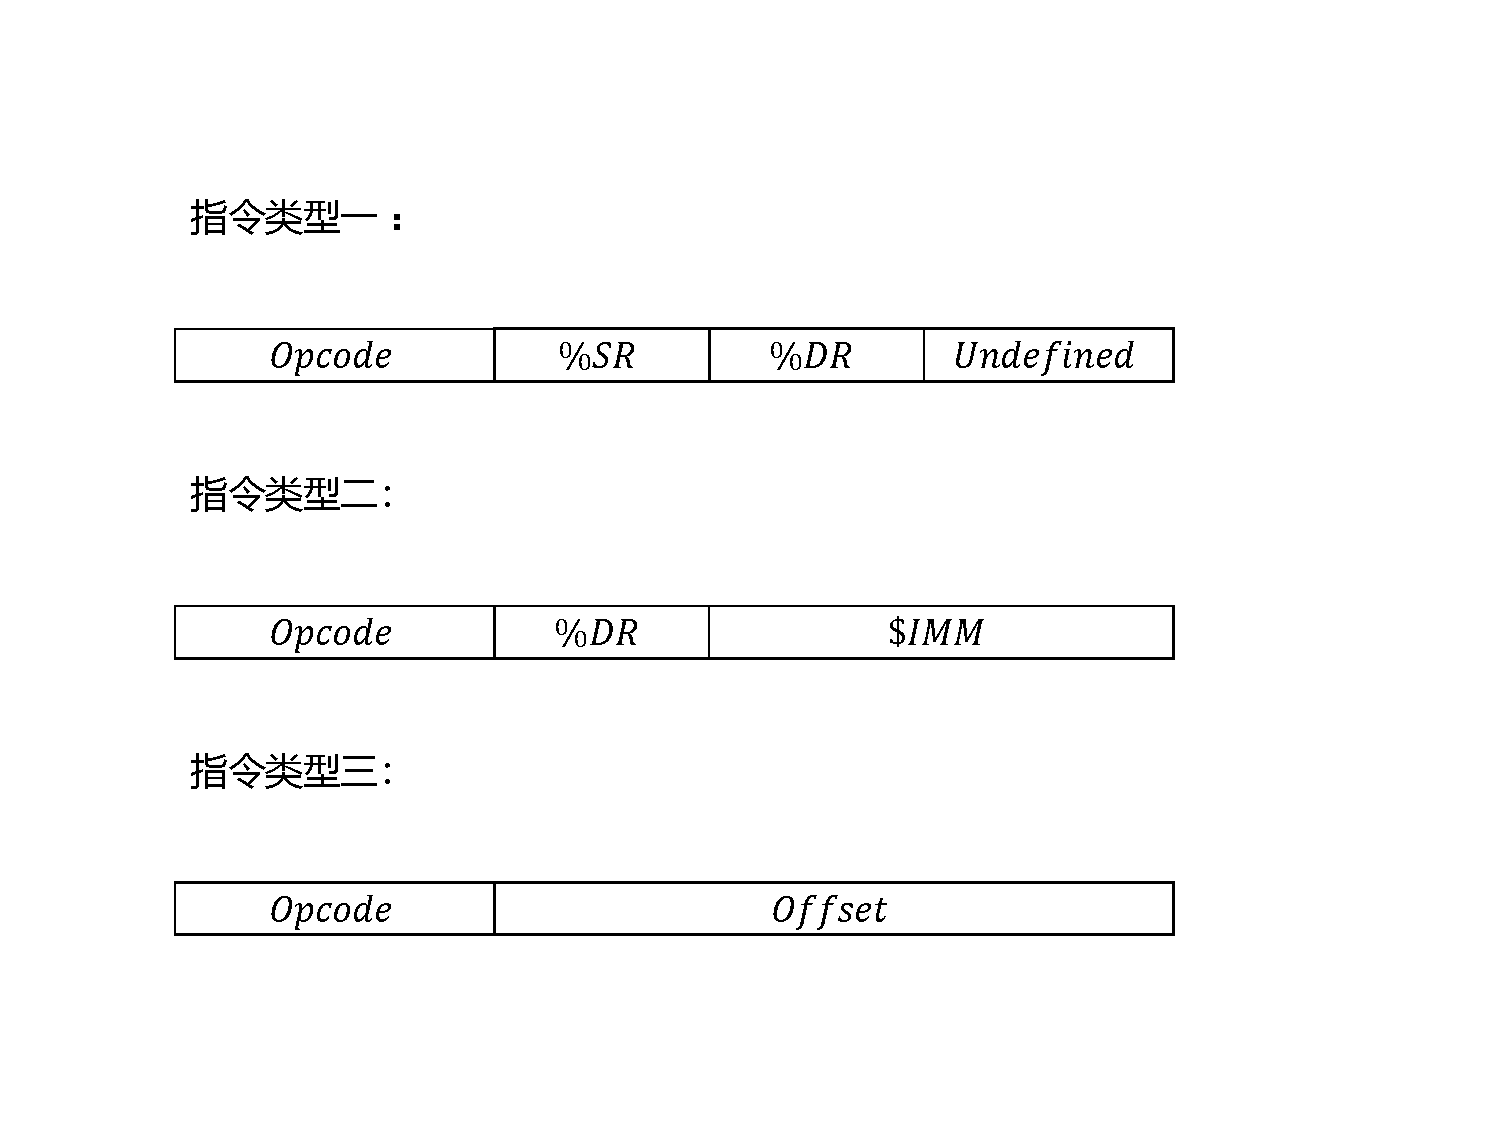
\includegraphics[scale=0.5]{2.pdf}
		\caption{指令格式类型}
	\end{figure}
	\section{实验器材和环境}
	\subsection{硬件}
	Nexys 4开发板
	\subsection{环境}
	运行在Windows 10下的Vivado 2016.4
	\section{实验设计思路}
	\subsection{RISC CPU的数据通路图}
	我们设计的CPU数据通路如下图所示:
	\begin{figure}[htb]
		\centering
		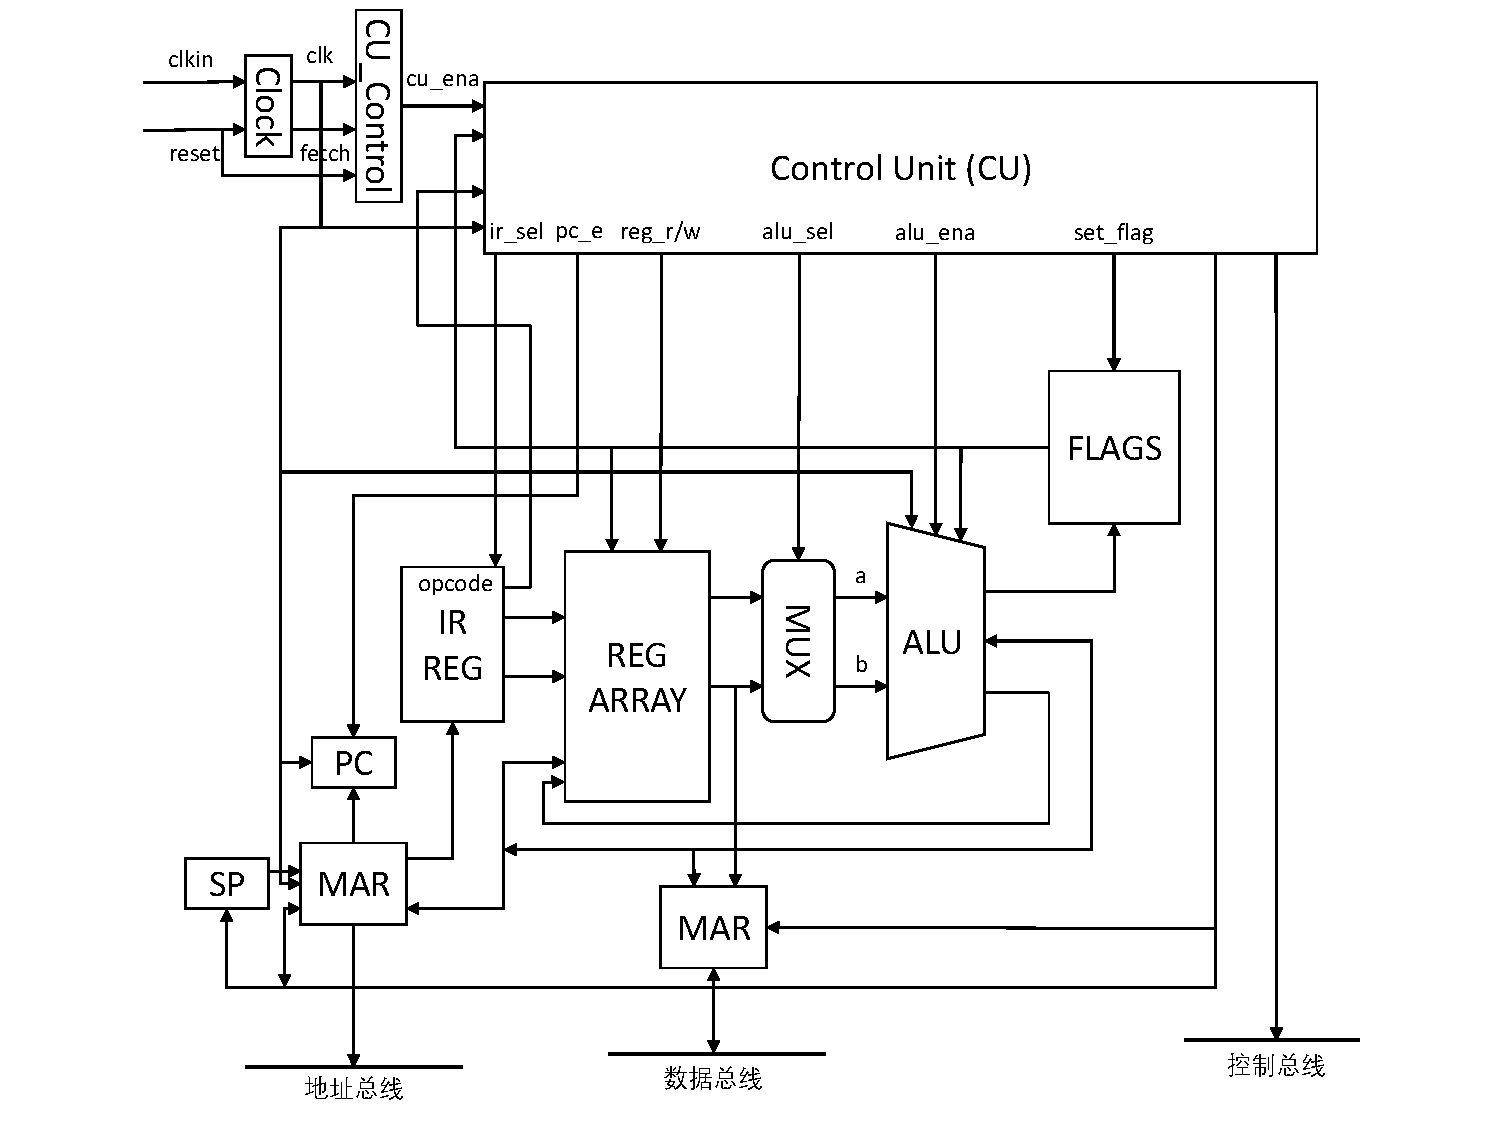
\includegraphics[scale=0.7]{3.pdf}
		\caption{CPU的数据通路}
	\end{figure}\par 
	我们在这个CPU中设计了8个16位的按照16位可读写的通用寄存器组(图中REG\_BANK)。除此之外,还包含指令寄存器(图中IR REG),地址寄存器(图中MAR),数据寄存器(图中MDR),栈指针寄存器(图中SP, Stack Pointer)以及标志寄存器(图中FLAG)。运算器为算术逻辑单元(图中ALU),负责进行数学运算和逻辑运算。程序计数器在图中为PC。控制部分为图中的Control Unit (CU),时钟信号由图中Clock发生。
	\subsection{模块划分}
	按照功能,我们将CPU划分为如下11个功能模块,下面逐个介绍这些模块的功能:
	\begin{enumerate}%	[(1)]
		\item 时钟发生器(Clock):时钟发生器的功能是根据外部时钟信号,产生一系列的特定时钟信号,送往其他部件,控制它们进行操作;
		\item 控制器(Control Unit, CU):控制器是CPU最核心的部件。CPU通过它来产生控制时序和控制信号,用来控制CPU中其他模块(例如ALU、寄存器)按照一定的时序关系工作。这一部分由两部分组成:状态机(CU)和状态机的控制器(CU\_Control);
		\item 指令寄存器(IR REG):指令寄存器用来存放当前正在执行的(PC指向的)指令;
		\item 通用寄存器组(REG ARRAY):这个寄存器组全部用于存储数据,它由8个16位寄存器组组成。此部件支持双端口读出、双端口写入操作。这些寄存器用来保存程序执行过程中需要的数据、中间变量和最后的结果,在访问时,必须一次性读出全部16位数据;
		\item 程序计数器(PC, Program Counter):程序计数器保存下一条指令的地址,CPU使用它在相应的ROM中取出指令;
		\item 算术逻辑运算器(ALU, Arithmetic and Logic Unit):算数逻辑运算器是一个16位定点运算器,支持基本的加减乘除、与或非等14算数、逻辑运算;
		\item 运算输入控制部件:此部件用来控制运算器的输入数据。送入ALU的数据只有两种:来自数据寄存器的16位数据和来自立即数的8位数据;
		\item 标志寄存器(FLAG):标志寄存器共有8位,但是只使用了4位。高4位未定义,低4位存储运算过程中产生的标志位。低4位由高到低依次为:进位(CF)、零(ZF)、溢出(OF)和符号(SF);
		\item 地址寄存器(MAR, Main Address Register):地址寄存器用来存储CPU访存时给出的地址,访存时的地址来源于此部件;
		\item 数据寄存器(MDR, Main Data Register):数据寄存器用来存储需要向地址总线输出的数据,或存储从总线上读取到的数据。它是双向输入输出的;
		\item 栈指针寄存器(SP, Stack Pointer):栈指针寄存器用于存储当前1的16位栈顶地址。每次出栈或入栈操作后,都要更新它的值。\par 
		这些模块的具体实现将在第五节介绍。
	\end{enumerate}
	\subsection{指令执行流程}
	为了更清楚的描述此CPU的运行过程,下面介绍指令的执行流程。总体上,所有指令的执行均包含3个阶段:取出指令、指令译码和取出操作数、执行和回写。这其中每个阶段又分为3个小阶段,所以执行中共经历了9个阶段。负责此模块实现的控制单元(CU)中的状态机也就在9个状态间进行转移。\par 
	\begin{enumerate}
		\item 算数逻辑运算指令:先把数据从寄存器中取出,然后经过运算器处理后再将结果写回寄存器,或设置相应的标志位。下面以带进位的加法指令ADC为例,介绍执行过程的各个阶段:\footnote{与ADC执行过程相似的指令还有:SBB, DIV, MUL, AND, NOT, OR, XOR, SHL, SHR, SAR, CMP, TEST和ADDI等。}
		\begin{figure}[H]
			\centering
			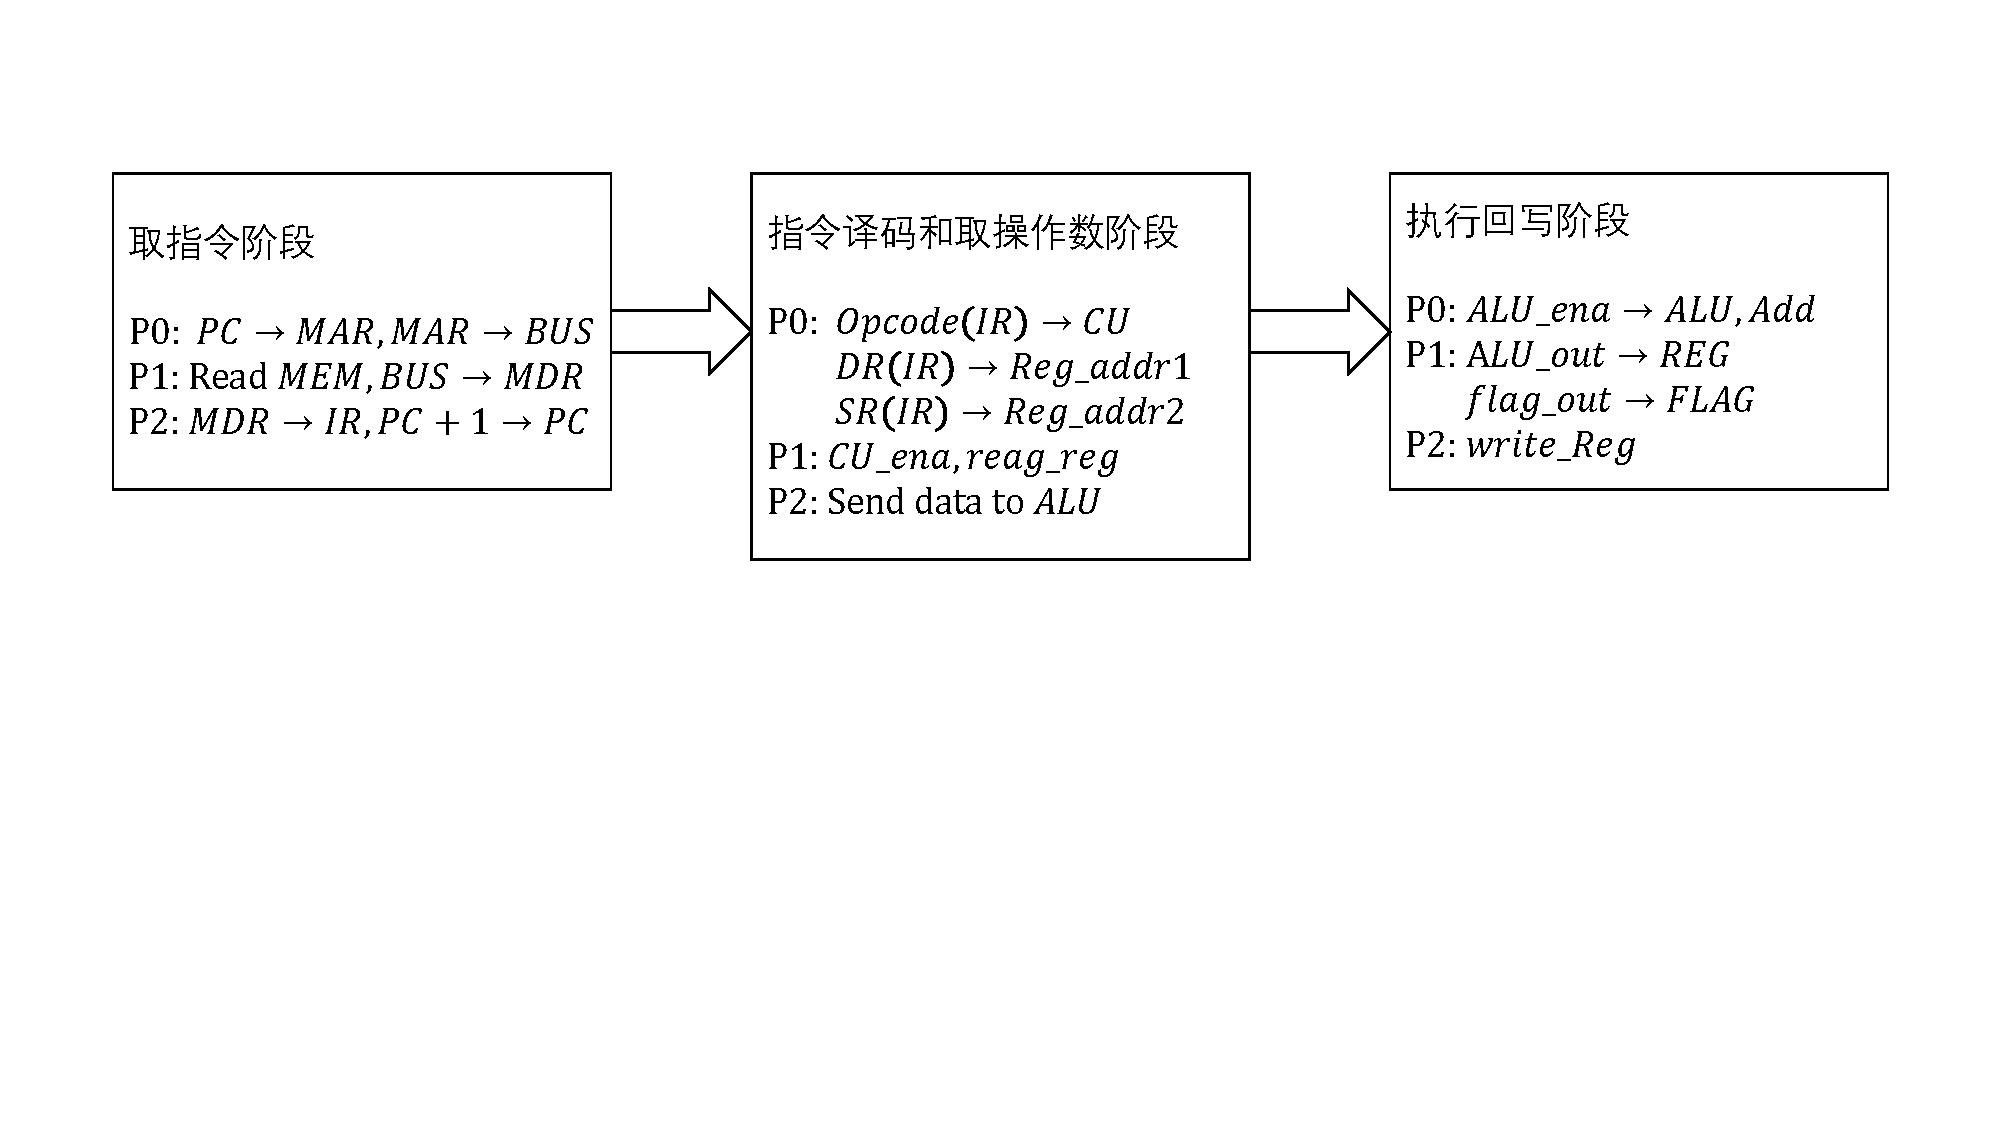
\includegraphics[scale=0.5]{4.pdf}
			\caption{算数和逻辑运算指令执行过程,以ADC为例}
		\end{figure}
		\item 数据传送类指令:此类指令包含在寄存器之间传输数据的MOV,寄存器的高8位或低8位的加载指令(MOVIH/L \$IMM, \%DR)。下面以寄存器间的传送指令MOV为例,介绍执行过程的各个阶段:
		\begin{figure}[H]
			\centering
			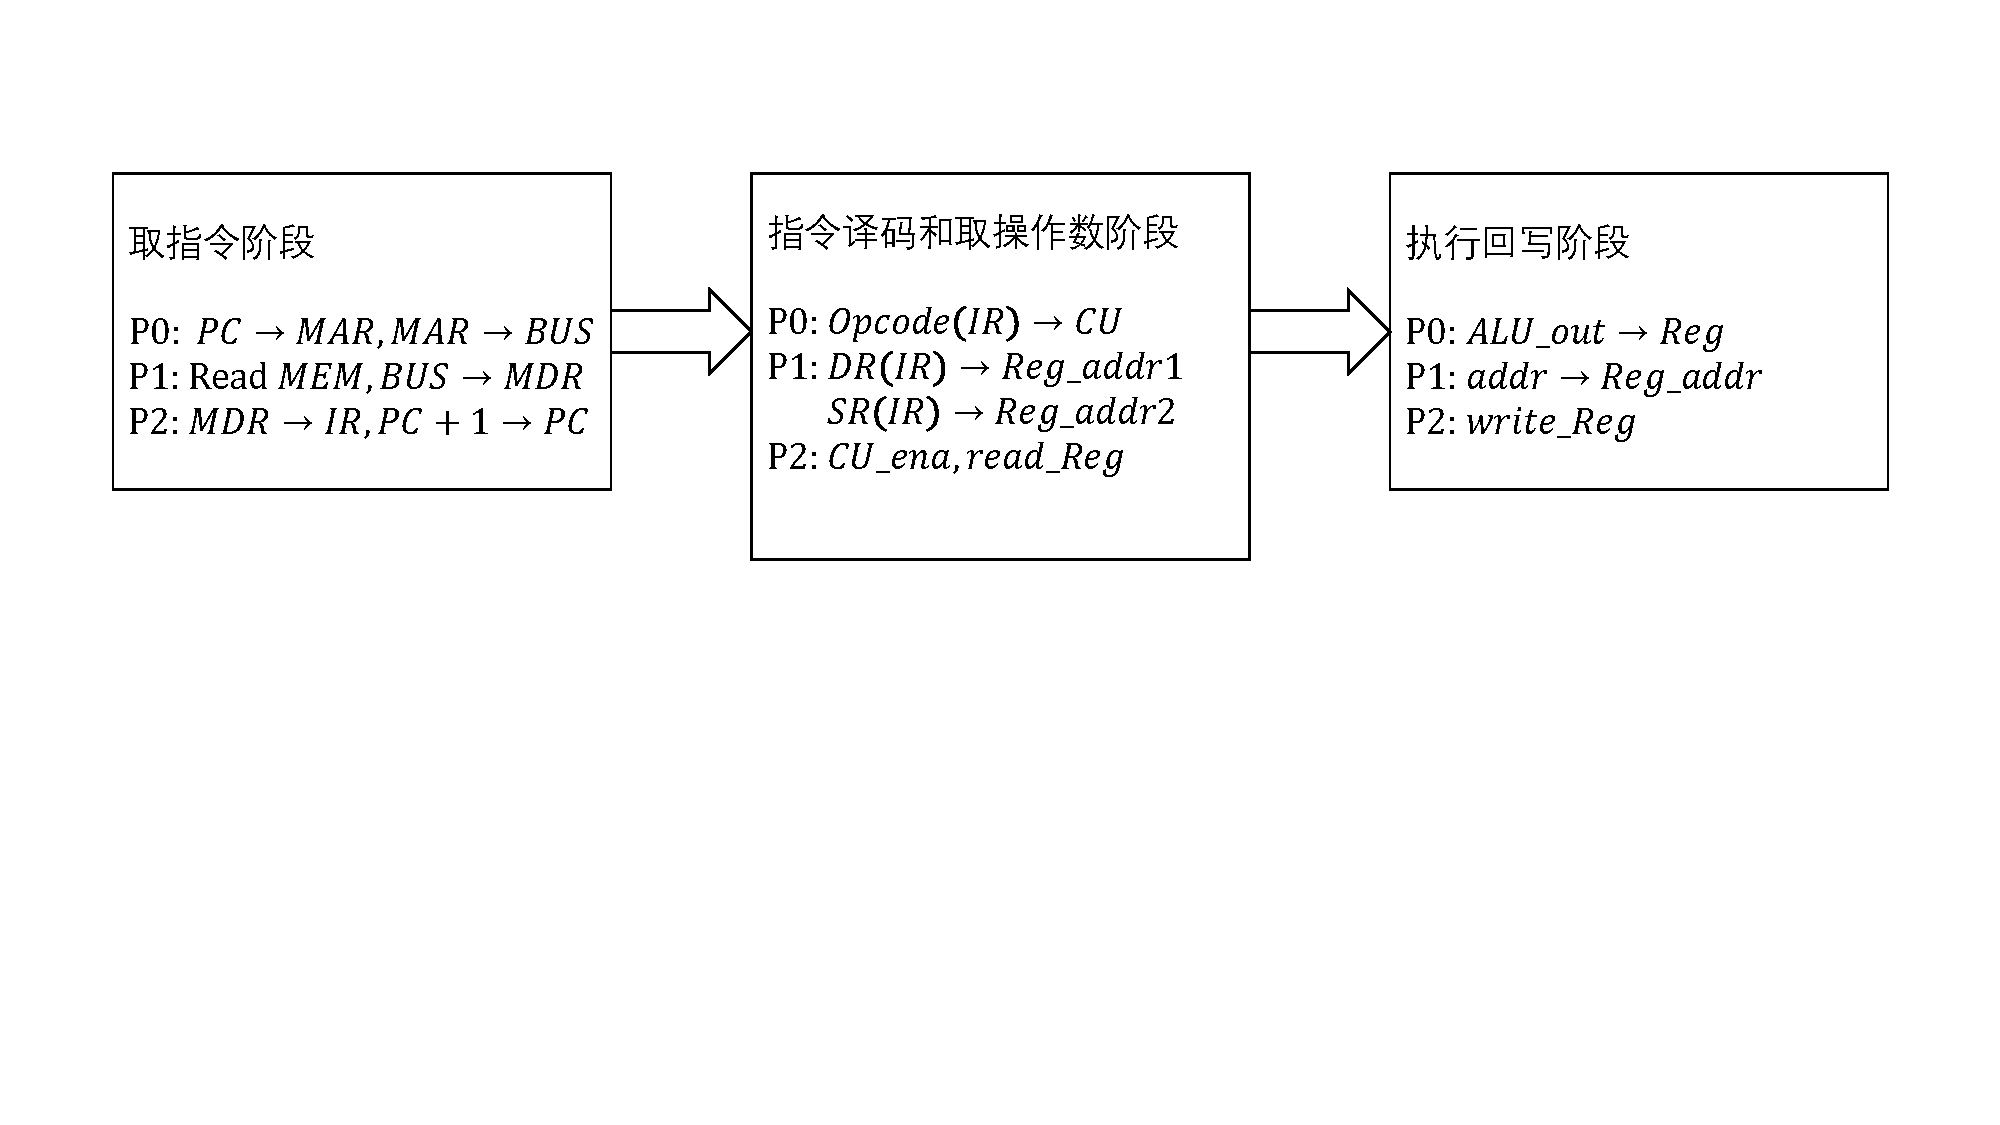
\includegraphics[scale=0.5]{5.pdf}
			\caption{数据传送类指令执行过程,以MOV为例}
		\end{figure}
		\item I/O类指令:此类指令包含写I/O端口指令(OUT \%SR, PORT)和读I/O端口指令(IN PORT, \%DR)。下面以OUT指令为例,介绍执行过程的各个阶段:
		\begin{figure}[H]
			\centering
			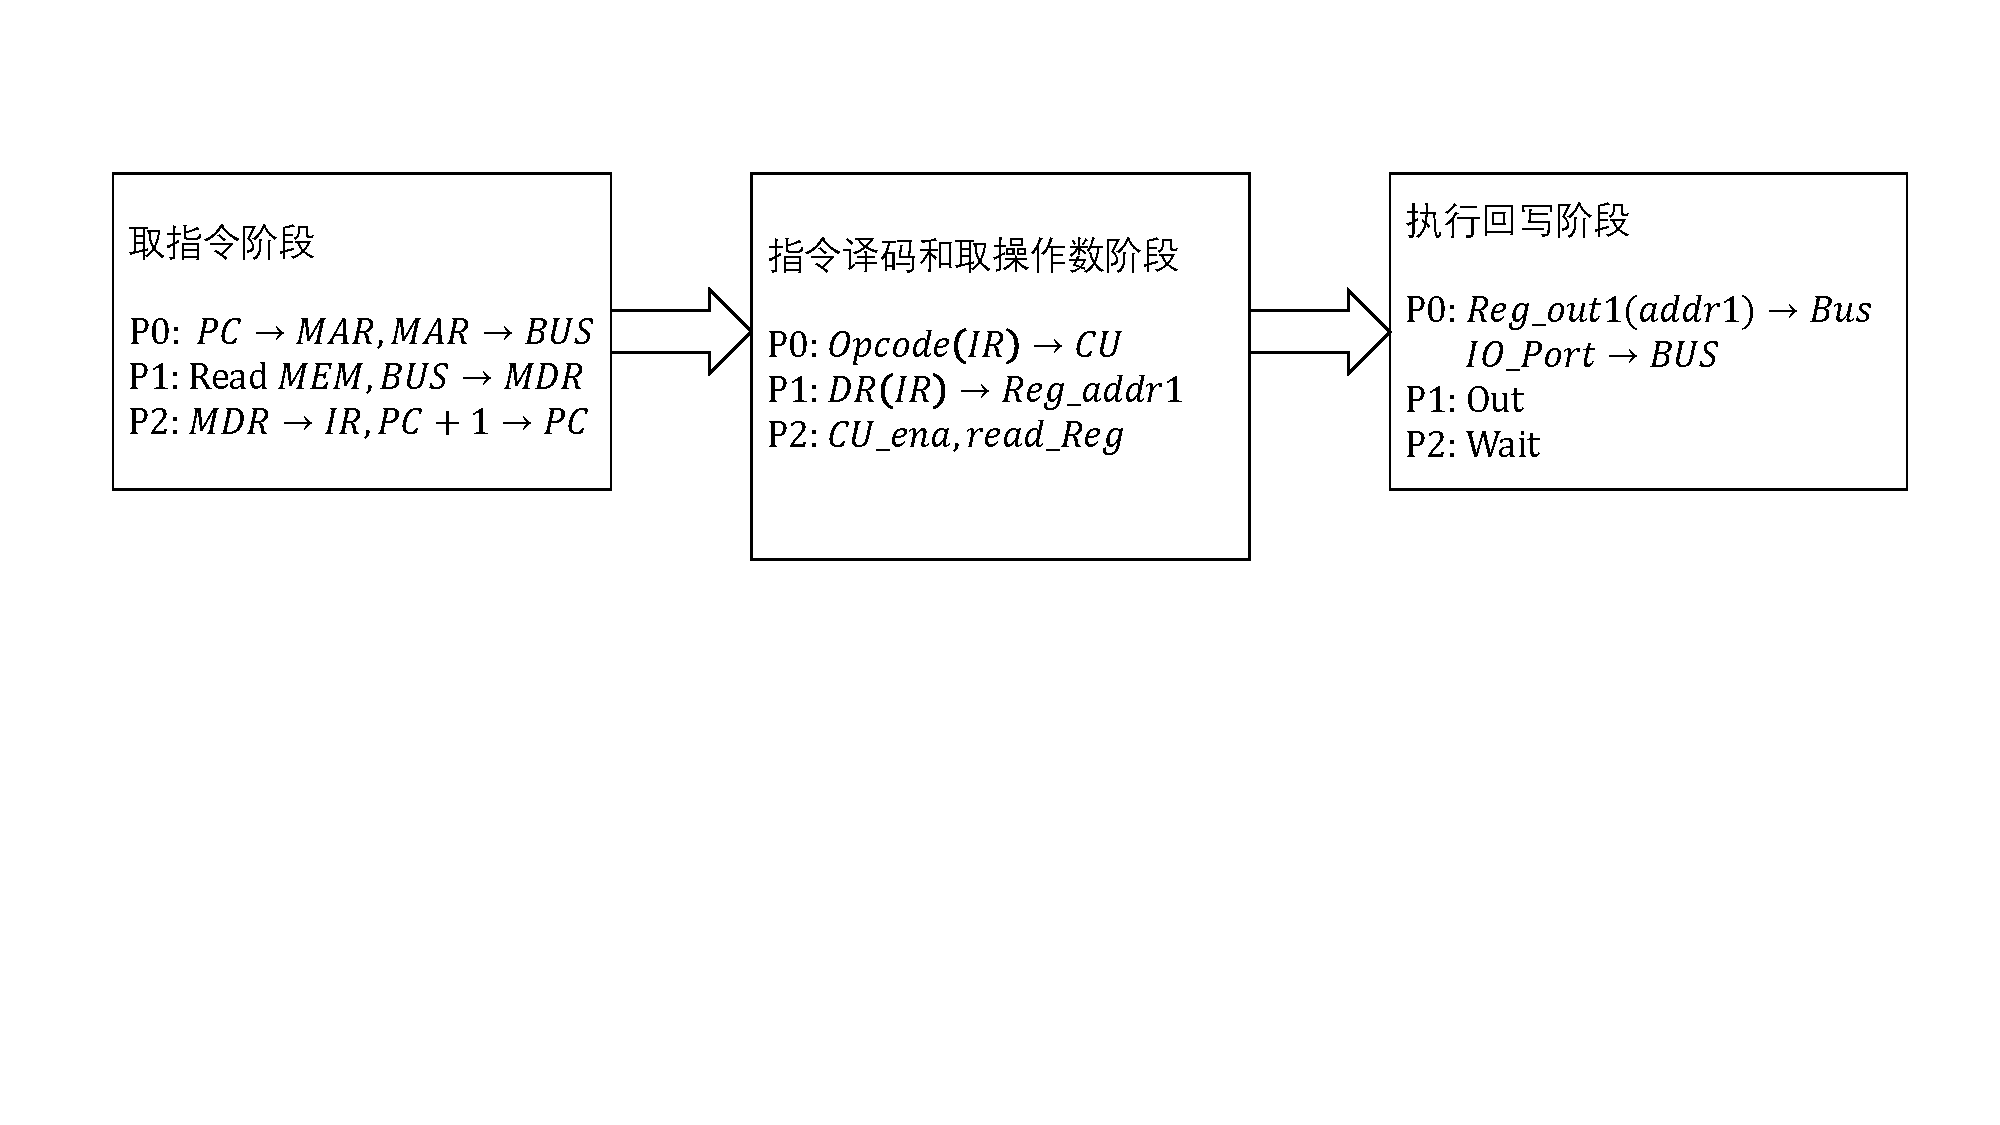
\includegraphics[scale=0.5]{6.pdf}
			\caption{I/O指令执行过程,以OUT为例}
		\end{figure}
		\item 控制转移类指令:可以分为有条件转移指令\footnote{此类指令包括JMPC, JNC, JMPZ和JNZ。}和无条件转移指令\footnote{此类指令为JMP}两大类。下面以JMPC为例,介绍执行过程的各个阶段:
		\begin{figure}[H]
			\centering
			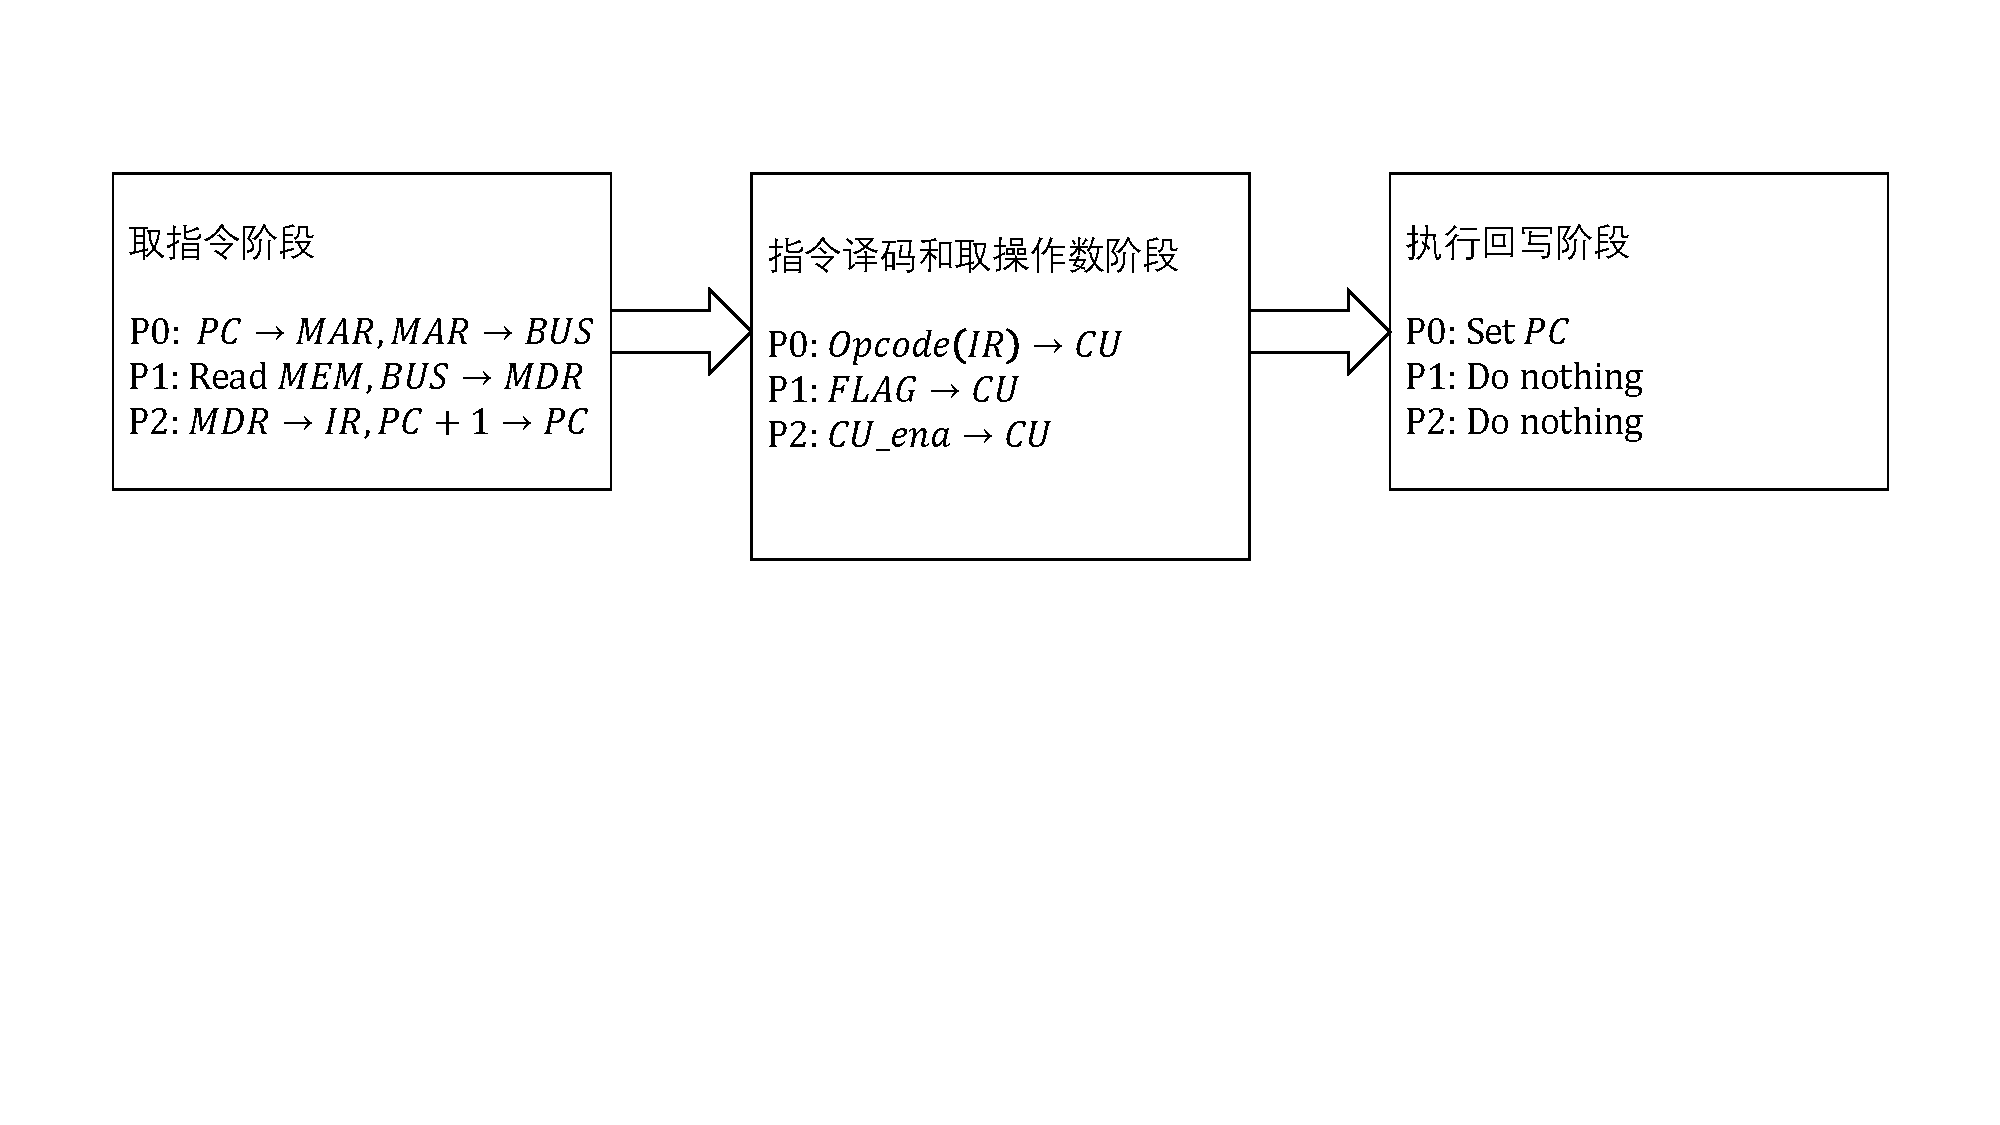
\includegraphics[scale=0.5]{7.pdf}
			\caption{条件转移类指令执行过程,以JMPC为例}
		\end{figure}
		\item 栈操作指令:包含入栈(PUSH \%SR)和出栈(POP \%DR)指令。下面以出栈指令POP为例,介绍执行过程的各个阶段:
		\begin{figure}[H]
			\centering
			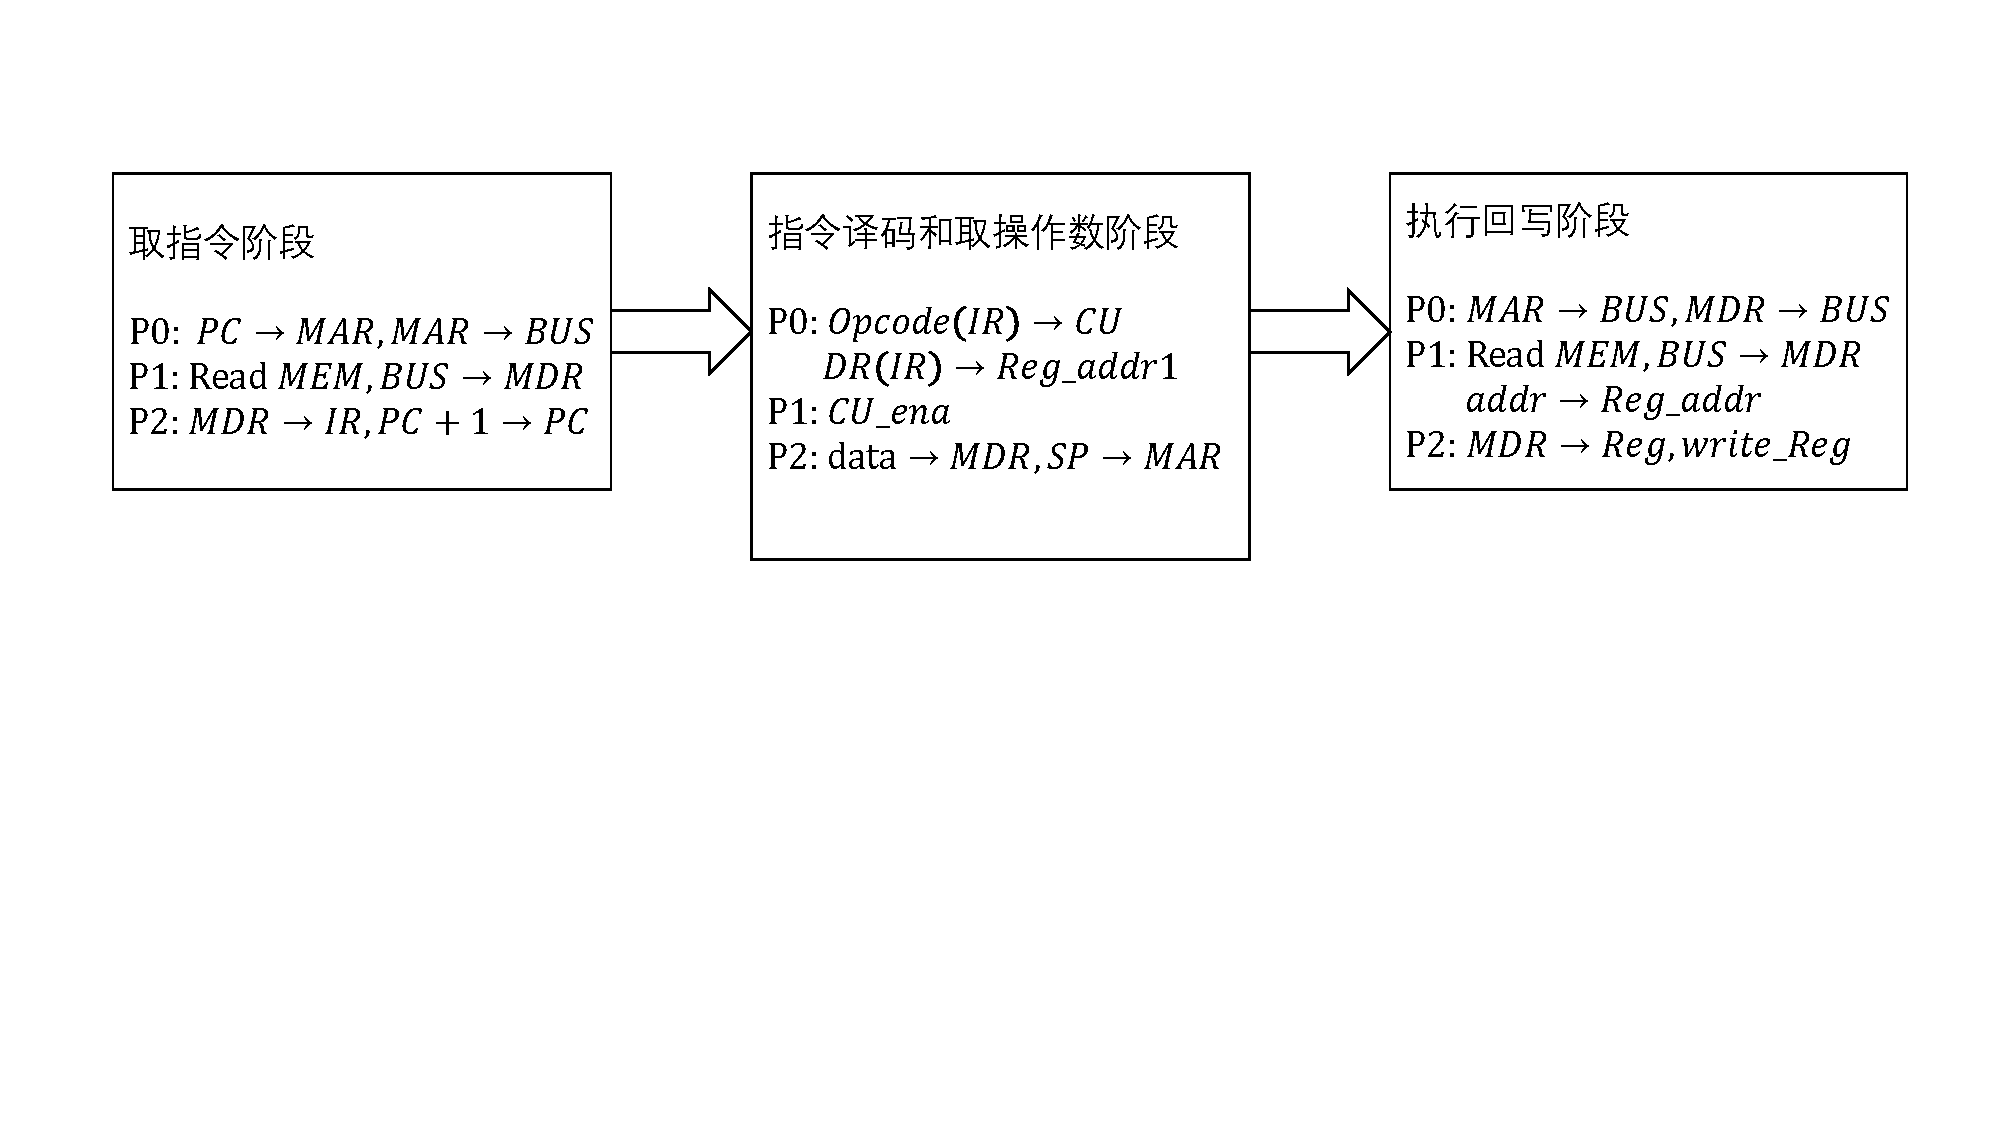
\includegraphics[scale=0.5]{8.pdf}
			\caption{栈操作指令执行过程,以POP为例}
		\end{figure}
		\item 访问内存类指令:包含取操作数指令(LOAD \%SR, \%DR)和存操作数指令(STORE \%SR, \%DR)。LOAD指令的作用是将源操作数寄存器中的数据当作地址,将这个内存地址中的数据装入目的寄存器\%DR;STORE指令的作用是将目的操作数寄存器中的数据当作地址,将源操作数中的数据存入此地址指向的内存。LOAD和STORE的执行过程分别如下所示:
		\begin{figure}[H]
			\centering
			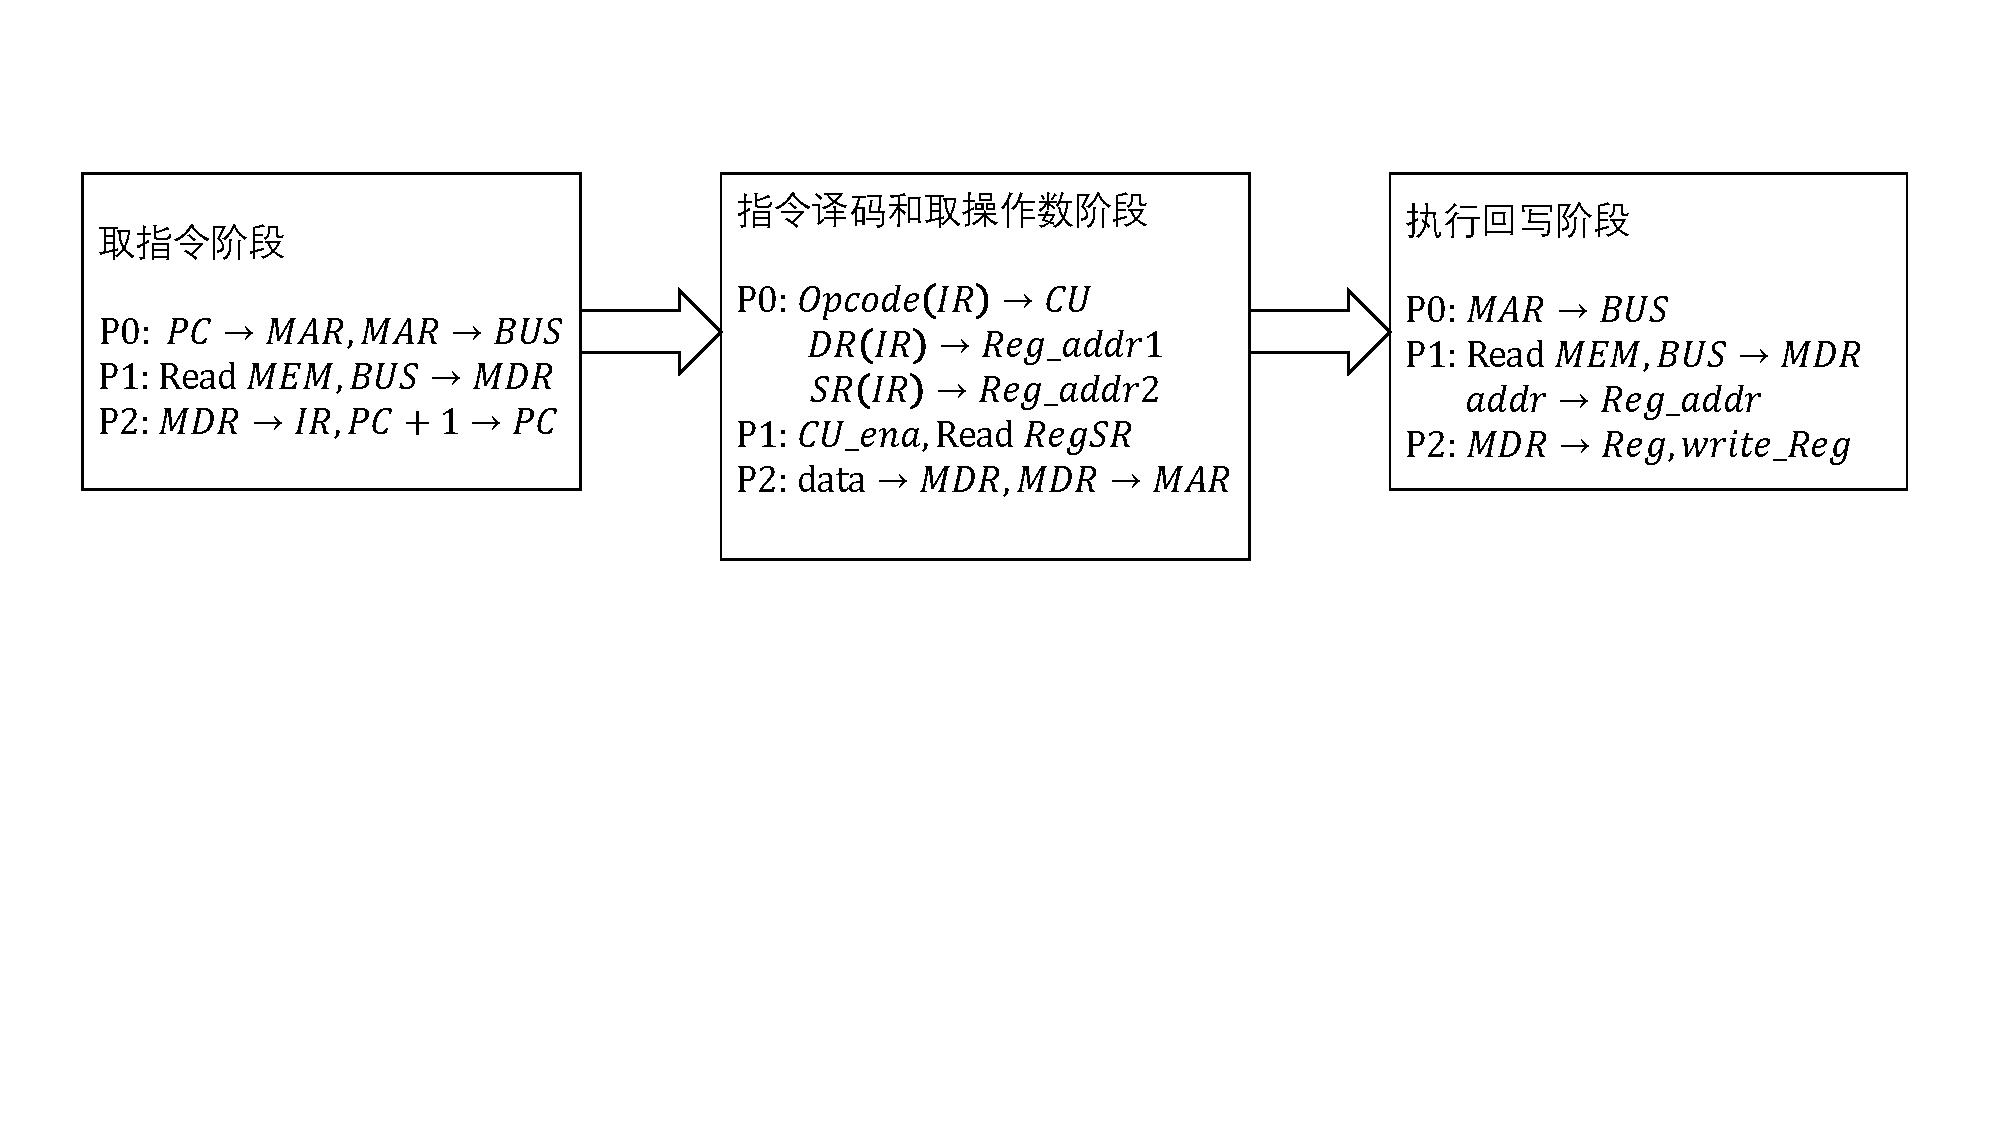
\includegraphics[scale=0.5]{9.pdf}
			\caption{LOAD指令执行过程}
		\end{figure}
		\begin{figure}[H]
			\centering
			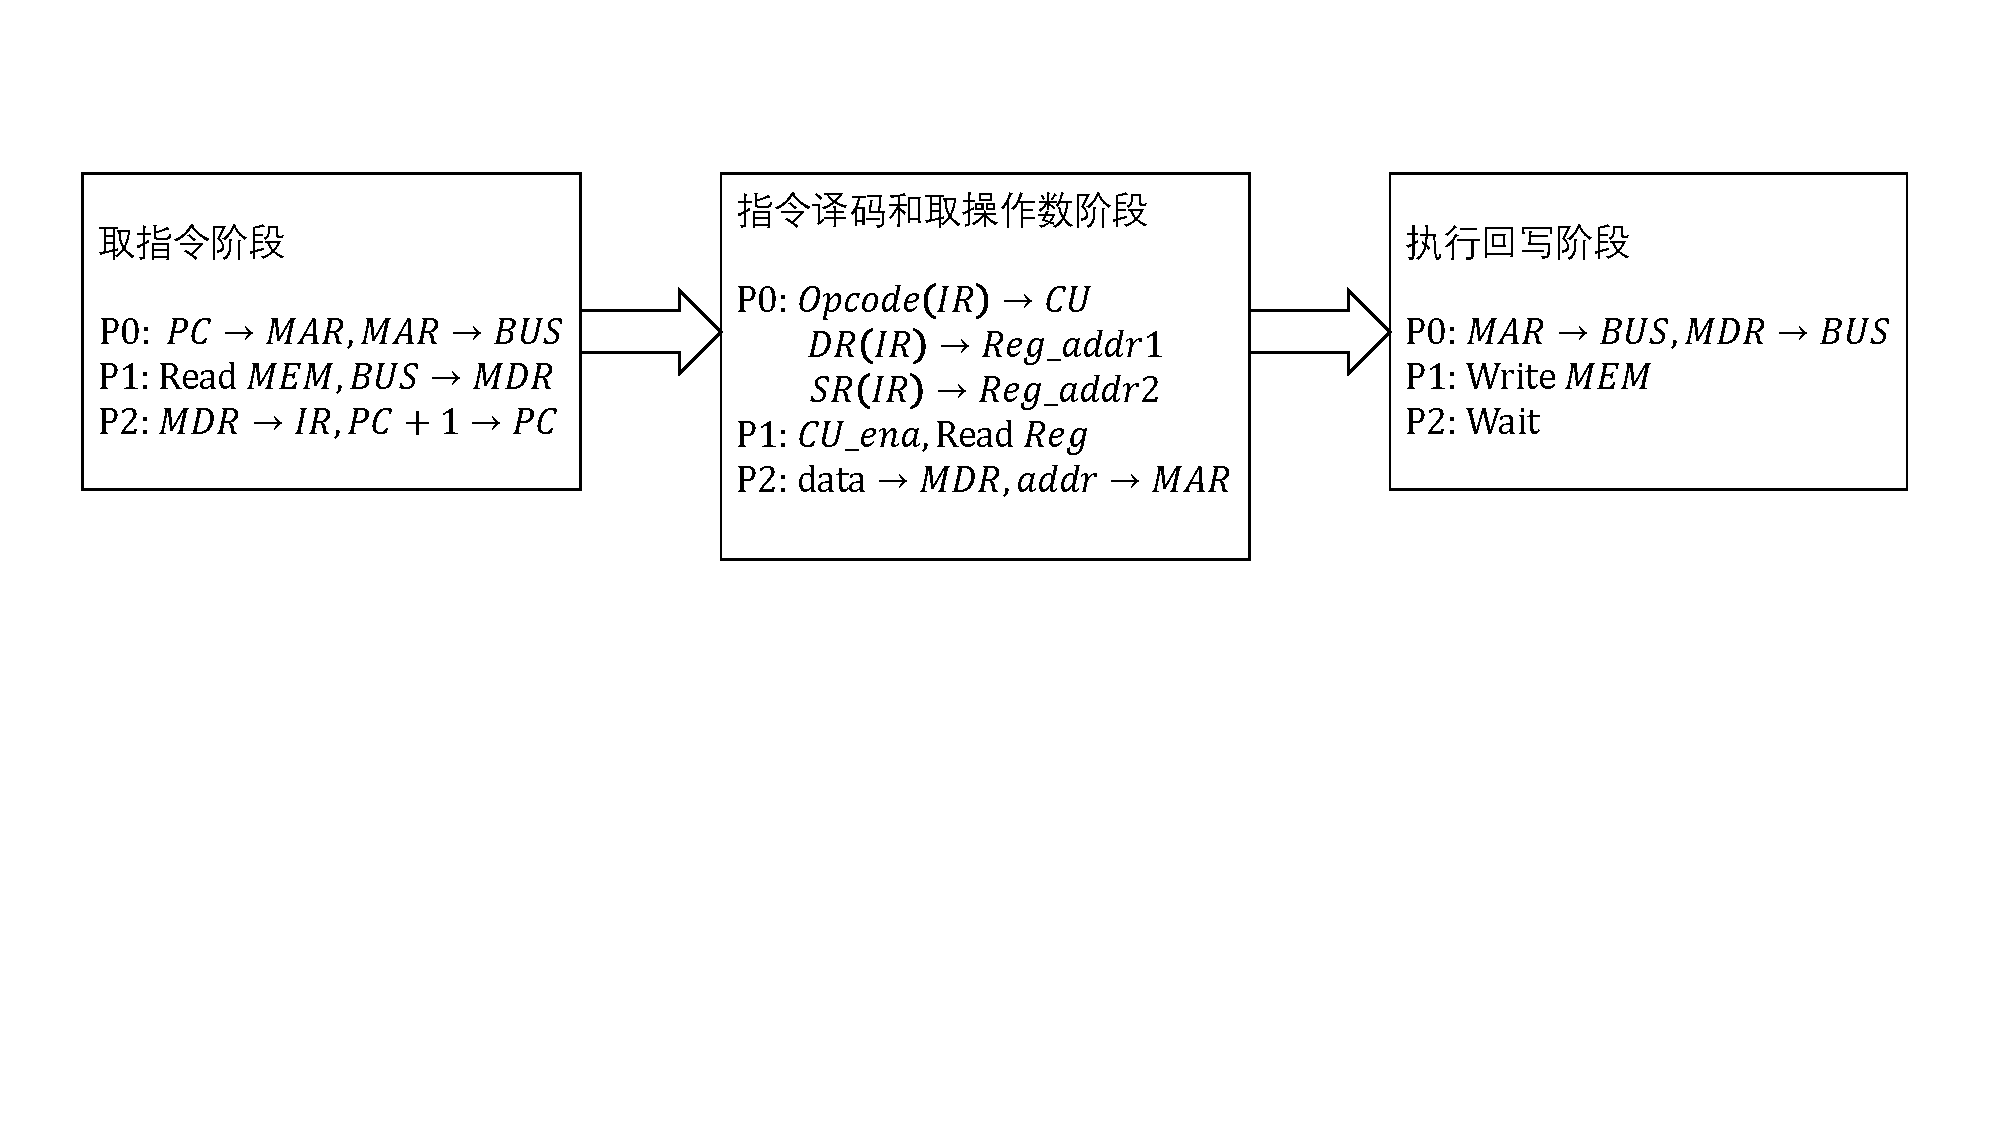
\includegraphics[scale=0.5]{10.pdf}
			\caption{STORE指令执行过程}
		\end{figure}
		\item 处理器控制类指令:包含空操作(NOP)和停机(HALT)两个指令。NOP不执行任何操作,只将PC增加1;HALT指令负责停止CPU的运行。它们的执行过程分别如下图所示:
			\begin{figure}[H]
			\centering
			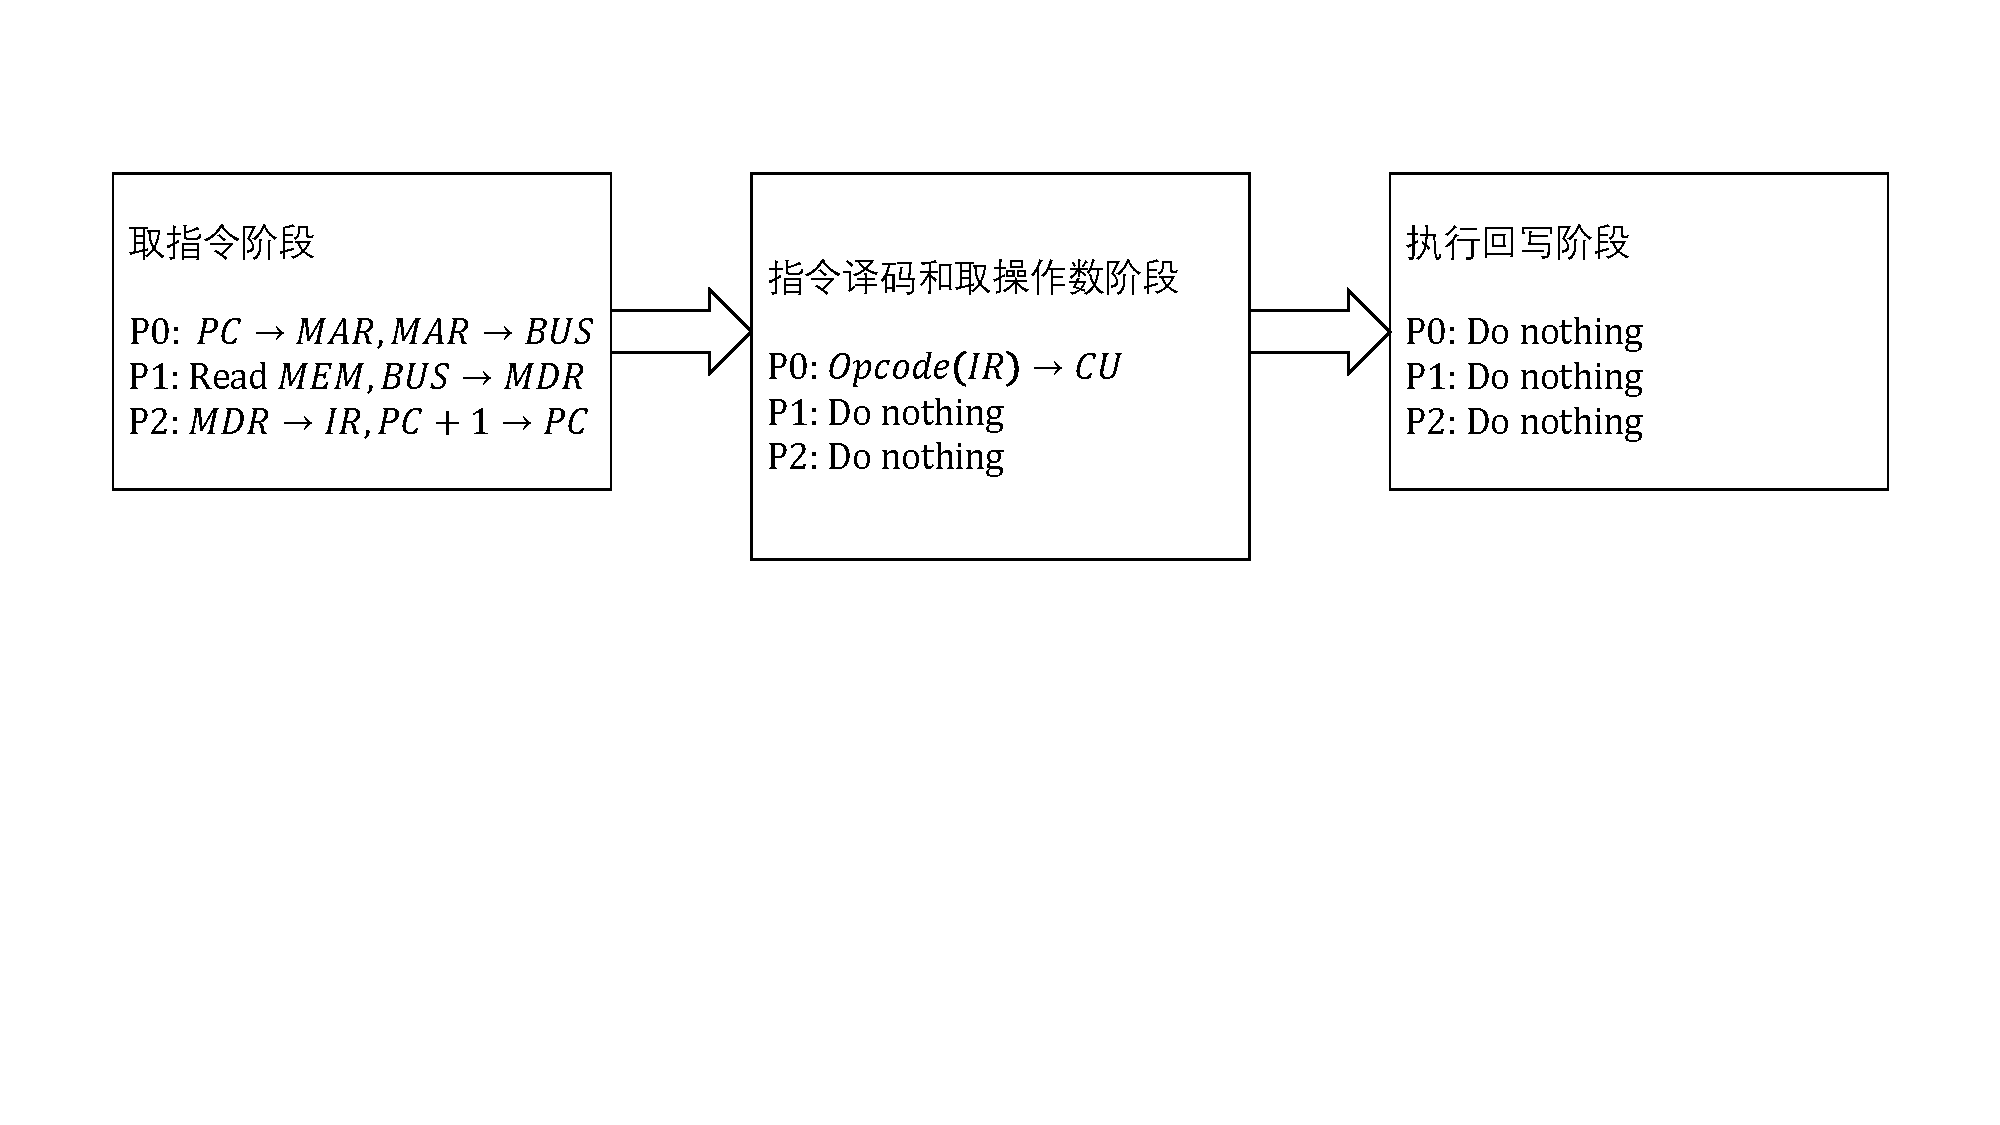
\includegraphics[scale=0.5]{11.pdf}
			\caption{NOP指令执行过程}
		\end{figure}
		\begin{figure}[H]
			\centering
			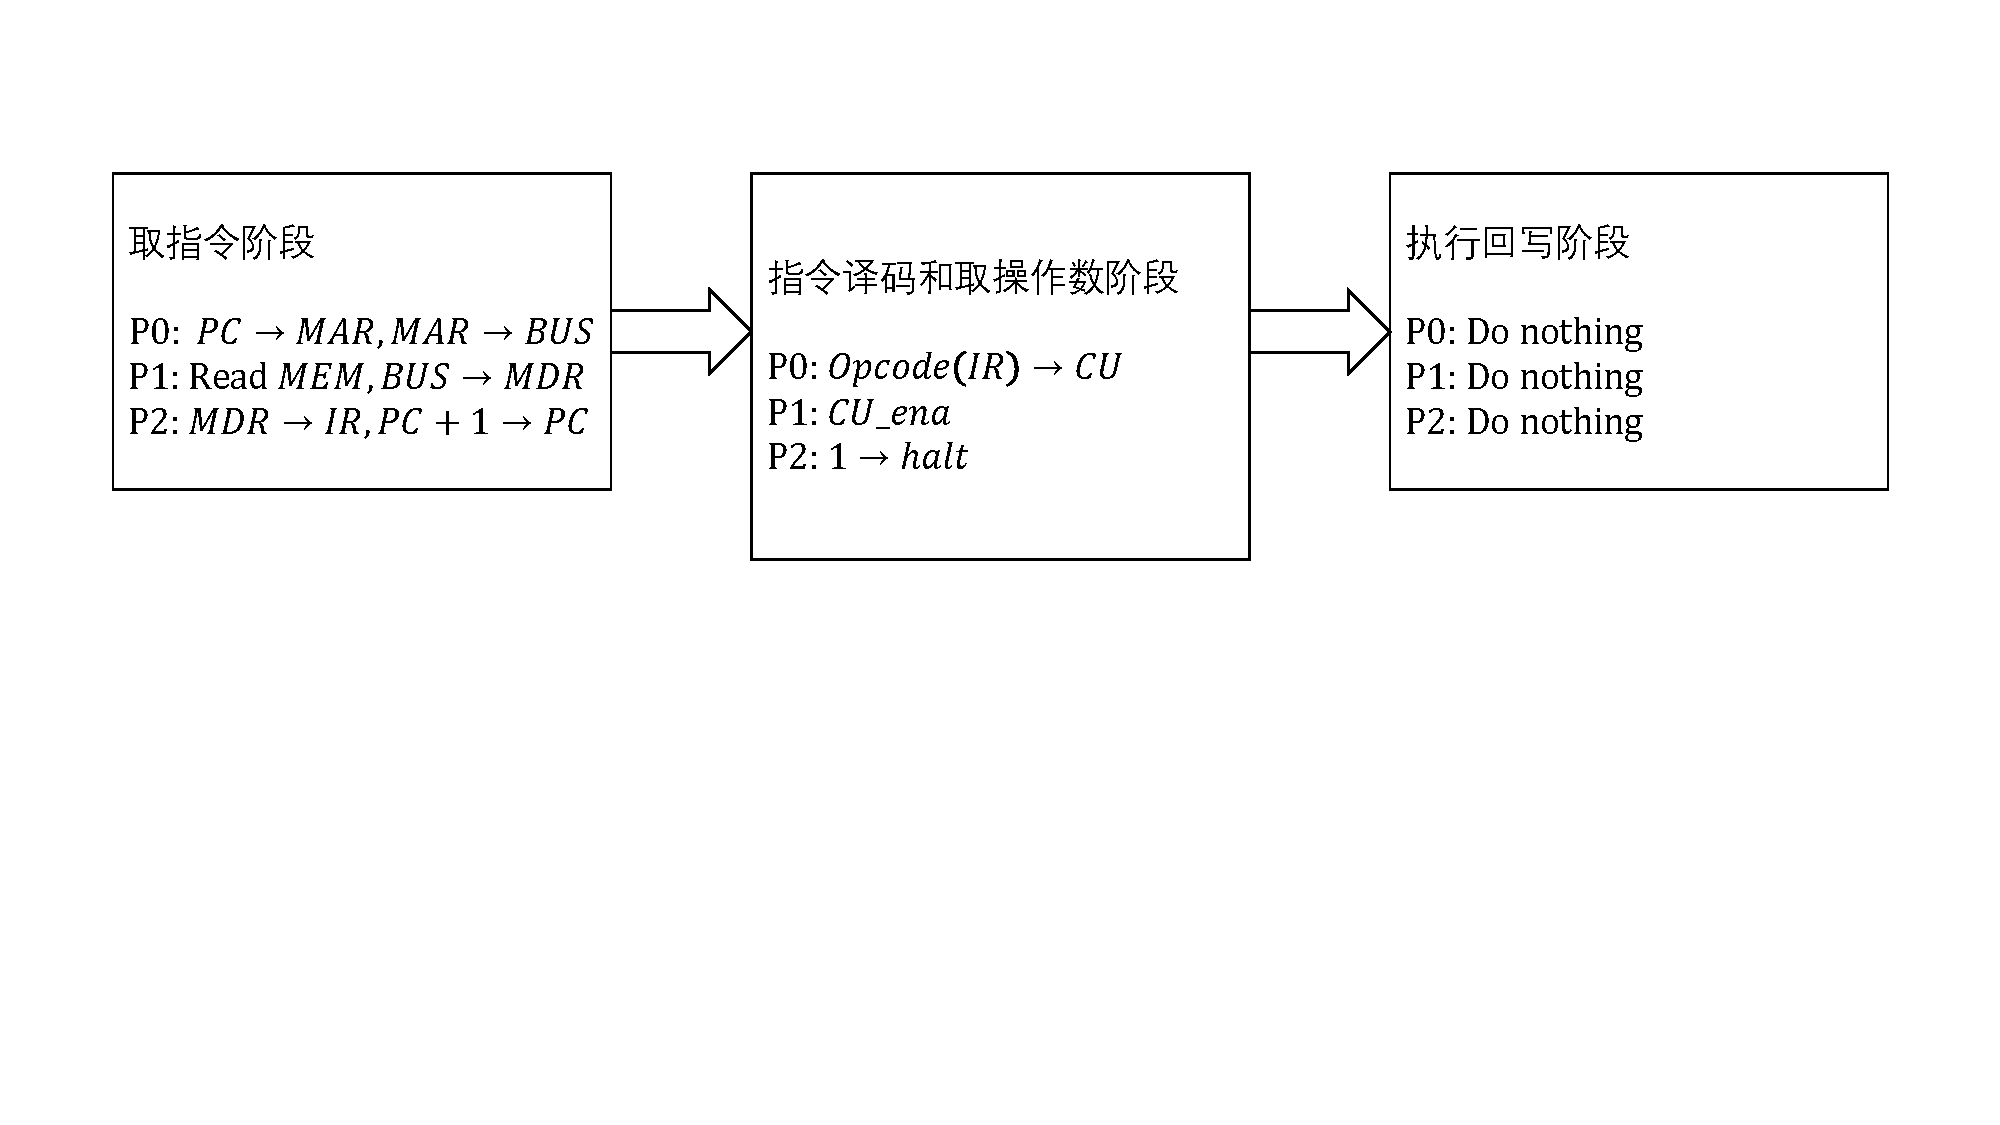
\includegraphics[scale=0.5]{12.pdf}
			\caption{HALT指令执行过程}
		\end{figure}
	\end{enumerate}
	\section{实验过程}
	本节介绍图3\footnote{第6页}中标出的各个模块的主要构成和\emph{Verilog HDL}代码实现。
		\subsection{时钟发生器}
		时钟发生器(Clock)模块利用外来的时钟信号$\id{clkin}$来生成一系列的时钟信号$\id{clkout},id{fetch}$送往CPU的其他部件。实现代码如下所示,为了简化CPU频率控制功能的实现,分成了分频器和时钟信号发生器。下面先说明分频器的信号端口:
		\begin{quote}
		输入信号:\\
		$\id{clkin}$——时钟信号;\\
		$\id{clkcon}$——频率控制信号;\\
		$\id{reset}$——复位信号。\\
		输出信号:\\
		$\id{clkout}$——分频后的时钟信号。
		\end{quote}\par 
		和时钟发生器的信号端口:
		\begin{quote}
		输入信号:\\
		$\id{clk}$——分频后的时钟信号;\\
		$\id{reset}$——复位信号。\\
		输出信号:\\
		$\id{clk\_r}$——$\id{clk}$取反后的时钟信号;\\
		$\id{fetch}$——$\id{clk}$的八分频,取指令信号。
		\end{quote}
		\begin{figure}[H] 
			\begin{minipage}[H]{0.5\linewidth}  
			\centerfirst
			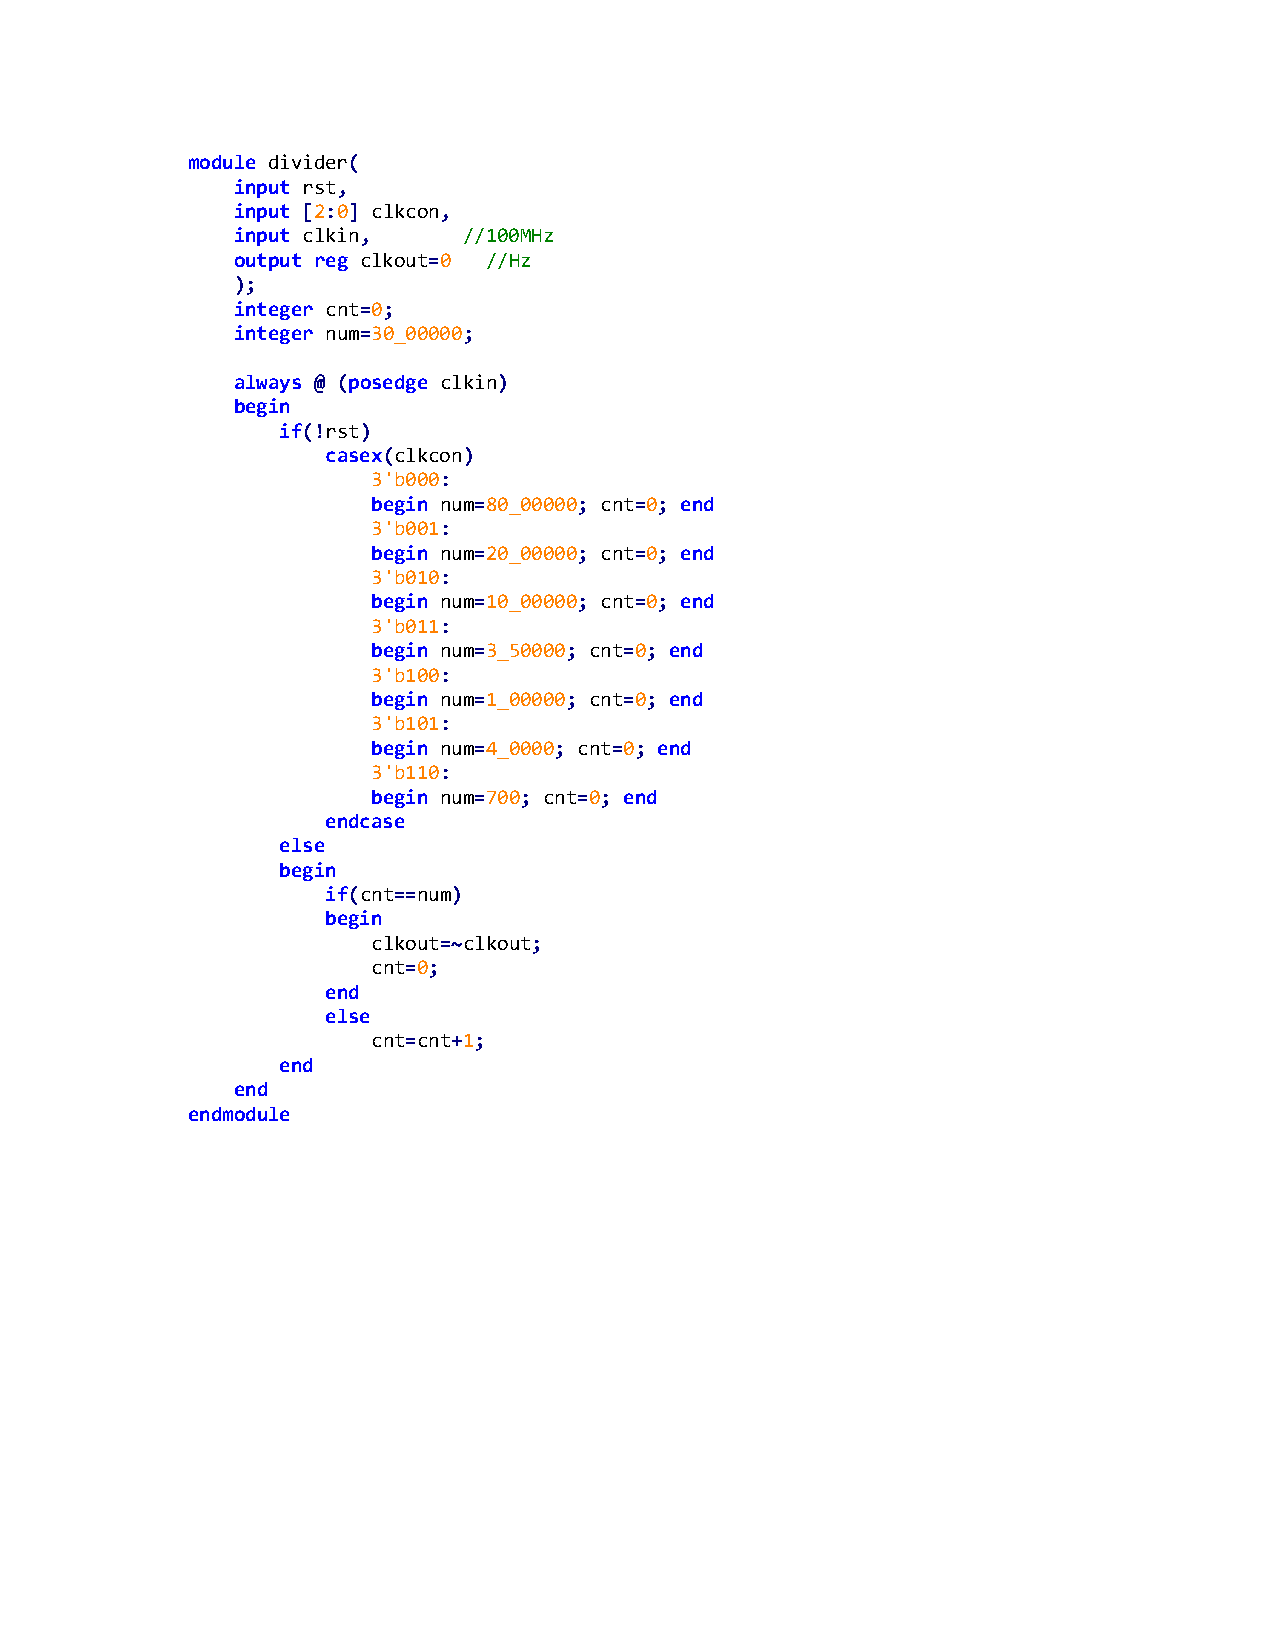
\includegraphics[scale=1]{13.pdf}  
			\caption*{}  
			%\label{fig:side:a}  
			\end{minipage}
			\begin{minipage}[H]{0.5\linewidth}  
			\centerfirst
			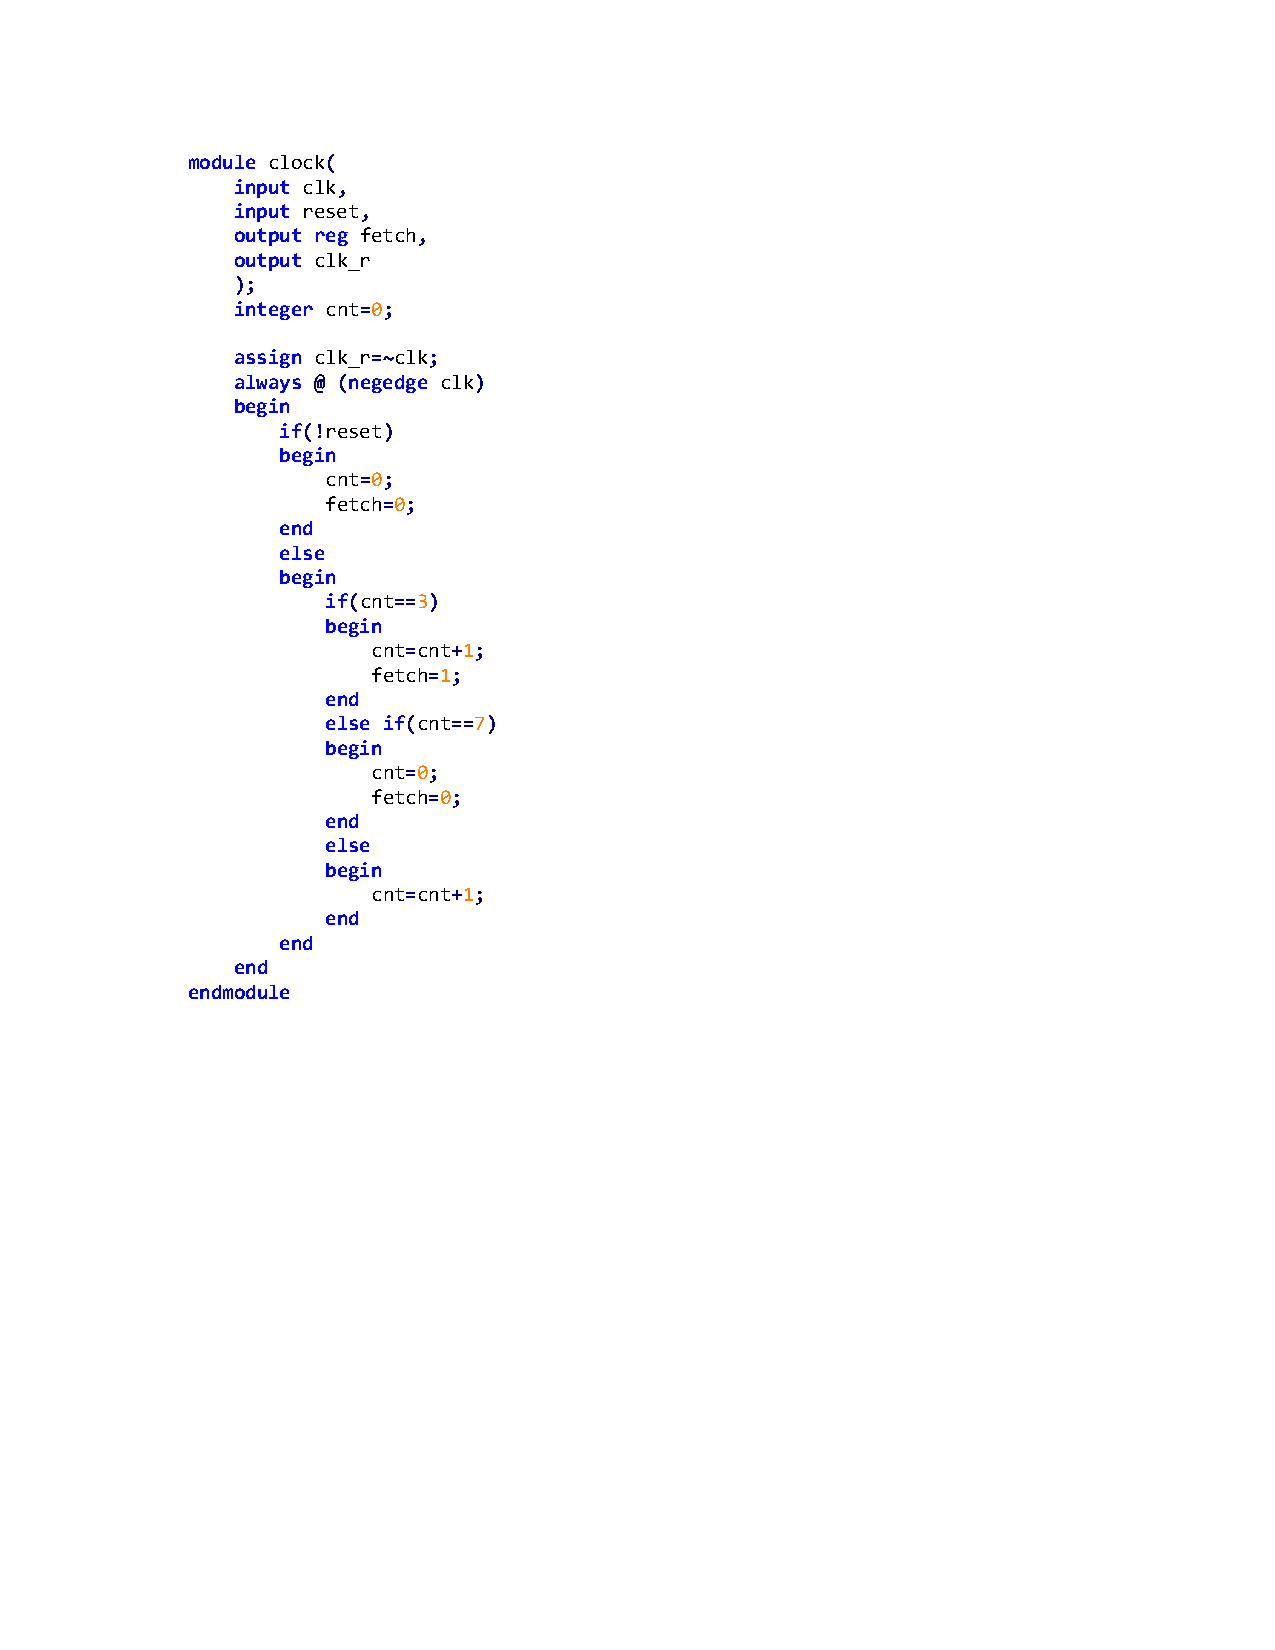
\includegraphics[scale=1]{14.pdf}  
			\caption*{}  
			%\label{fig:side:b}  
			\end{minipage}
			\caption*{代码1: 时钟模块}  
		\end{figure} 
		下面是此时钟发生器的模块符号,以及仿真结果。
		\begin{figure}[H]
			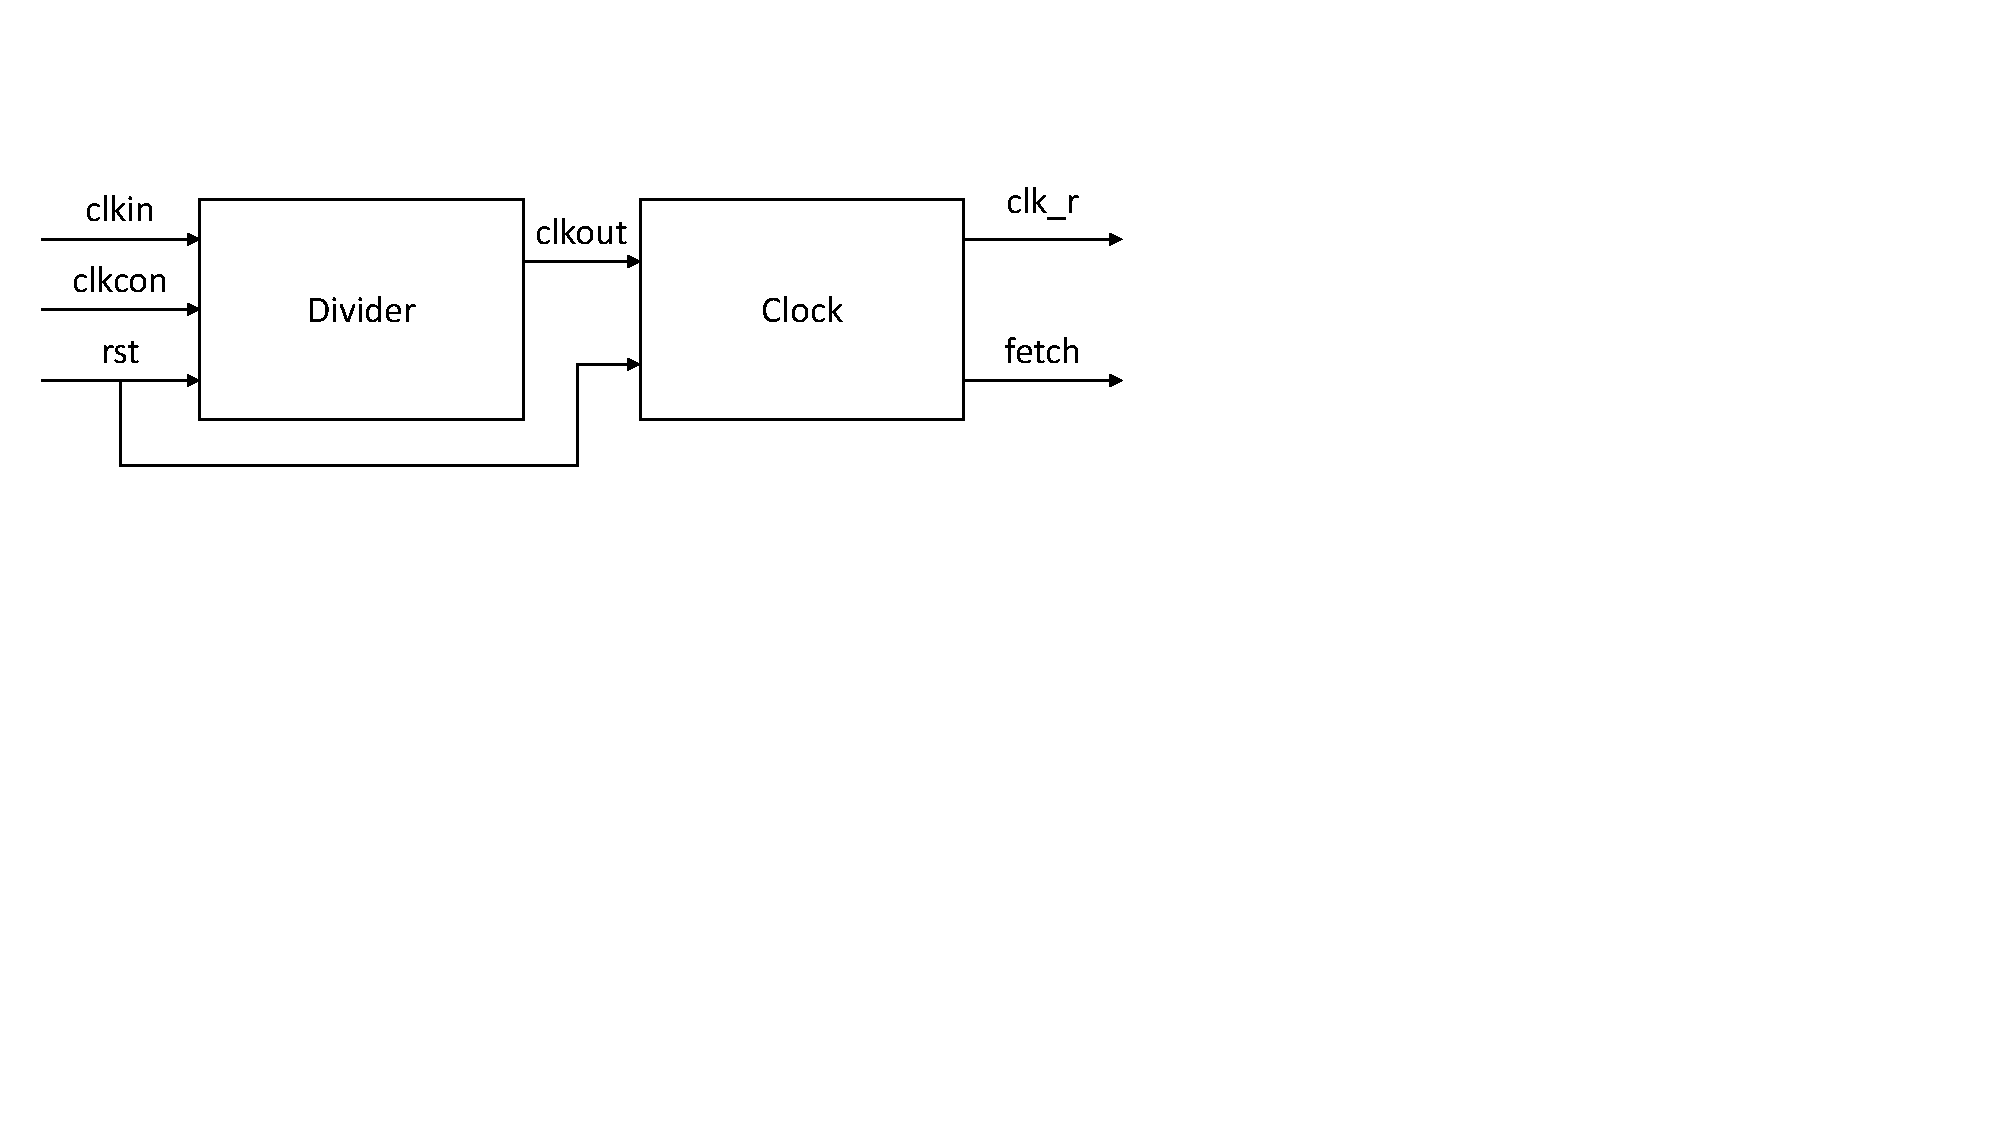
\includegraphics[scale=0.5]{15.pdf}
			\caption{时钟模块符号}
		\end{figure}
		\subsection{程序计数器}
		程序计数器(PC, Program Counter)用于提供执行指令的地址。指令按顺序存放在存储器(ROM)中,在控制器的控制下按顺序读取并执行指令。CPU的控制逻辑有两种生成指令地址的方法:
		\begin{enumerate}[(1)]
			\item 顺序执行时,$\id{PC}\gets \id{PC}+1$(规定每条指令长度都为1个字,16位);
			\item 需要跳转时,根据跳转指令改变PC的值。
		\end{enumerate}
		\par 端口说明如下:
		\begin{quote}
			输入信号:\\
		    $\id{clk}$——时钟信号;\\
		    $\id{rst}$——复位信号;\\
		    $\id{offset}$——转移时的偏移量;\\
		    $\id{pc\_inc}$——自增1控制信号(低电平时PC加1);\\
		    $\id{pc\_ena}$——PC更新使能信号;\\
		    $\id{sw}$——程序选择信号。\\
		    输出信号:\\
		    $\id{pc\_value}$——PC的值,即指令地址。
		\end{quote}\par 
		复位(rst置高位后),$\id{PC}\gets \id{sw}\times 32+10$. 即每次CPU重新启动时,将根据程序选择信号sw读取相应起始地址中的指令,然后执行。在指令执行阶段,译码过后根据指令内容对程序计数器进行更新。如果执行的是跳转指令,则控制器(CU)根据标志寄存器(FLAGS)中的相关状态位来判断是否发生跳转,具体过程如下表所示。如果需要发生跳转,控制器将pc\_ena和pc\_inc信号输出为高电位,PC的值在本模块中得到更新;如果跳转条件不满足或不是跳转指令,则CU将pc\_ena置位高电位,pc\_inc置为低电位,此时PC自增1。
		% Please add the following required packages to your document preamble:
		% \usepackage{multirow}
		\begin{table}[htb]
			\centering
			\caption{指令操作码与指令寄存器更新的逻辑关系}
			\begin{tabular}{c|c|c|c|c|c}
				指令                    & 操作码                    & 零标识ZF & 进位标志CF & 是否跳转 & 更新后的PC值                            \\ \hline
				JMP                   & 10111                  & X     & X      & 是    & $\id{PC}\gets \id{PC}+\id{offset}$ \\ \hline
				\multirow{2}{*}{JMPC} & \multirow{2}{*}{11000} & X     & 0      & 否    & $\id{PC}\gets \id{PC}+1$           \\ \cline{3-6} 
				&                        & X     & 1      & 是    & $\id{PC}\gets \id{PC}+\id{offset}$ \\ \hline
				\multirow{2}{*}{JNC}  & \multirow{2}{*}{11001} & X     & 0      & 是    & $\id{PC}\gets \id{PC}+\id{offset}$ \\ \cline{3-6} 
				&                        & X     & 1      & 否    & $\id{PC}\gets \id{PC}+1$           \\ \hline
				\multirow{2}{*}{JMPZ} & \multirow{2}{*}{11010} & 0     & X      & 否    & $\id{PC}\gets \id{PC}+1$           \\ \cline{3-6} 
				&                        & 1     & X      & 是    & $\id{PC}\gets \id{PC}+\id{offset}$ \\ \hline
				\multirow{2}{*}{JNZ}  & \multirow{2}{*}{11011} & 0     & X      & 是    & $\id{PC}\gets \id{PC}+\id{offset}$ \\ \cline{3-6} 
				&                        & 1     & X      & 否    & $\id{PC}\gets \id{PC}+1$           \\ \hline
				其他                    & --                     & X     & X      & 否    & $\id{PC}\gets \id{PC}+1$          
			\end{tabular}
		\end{table}
		\begin{figure}[H]
			\centering
			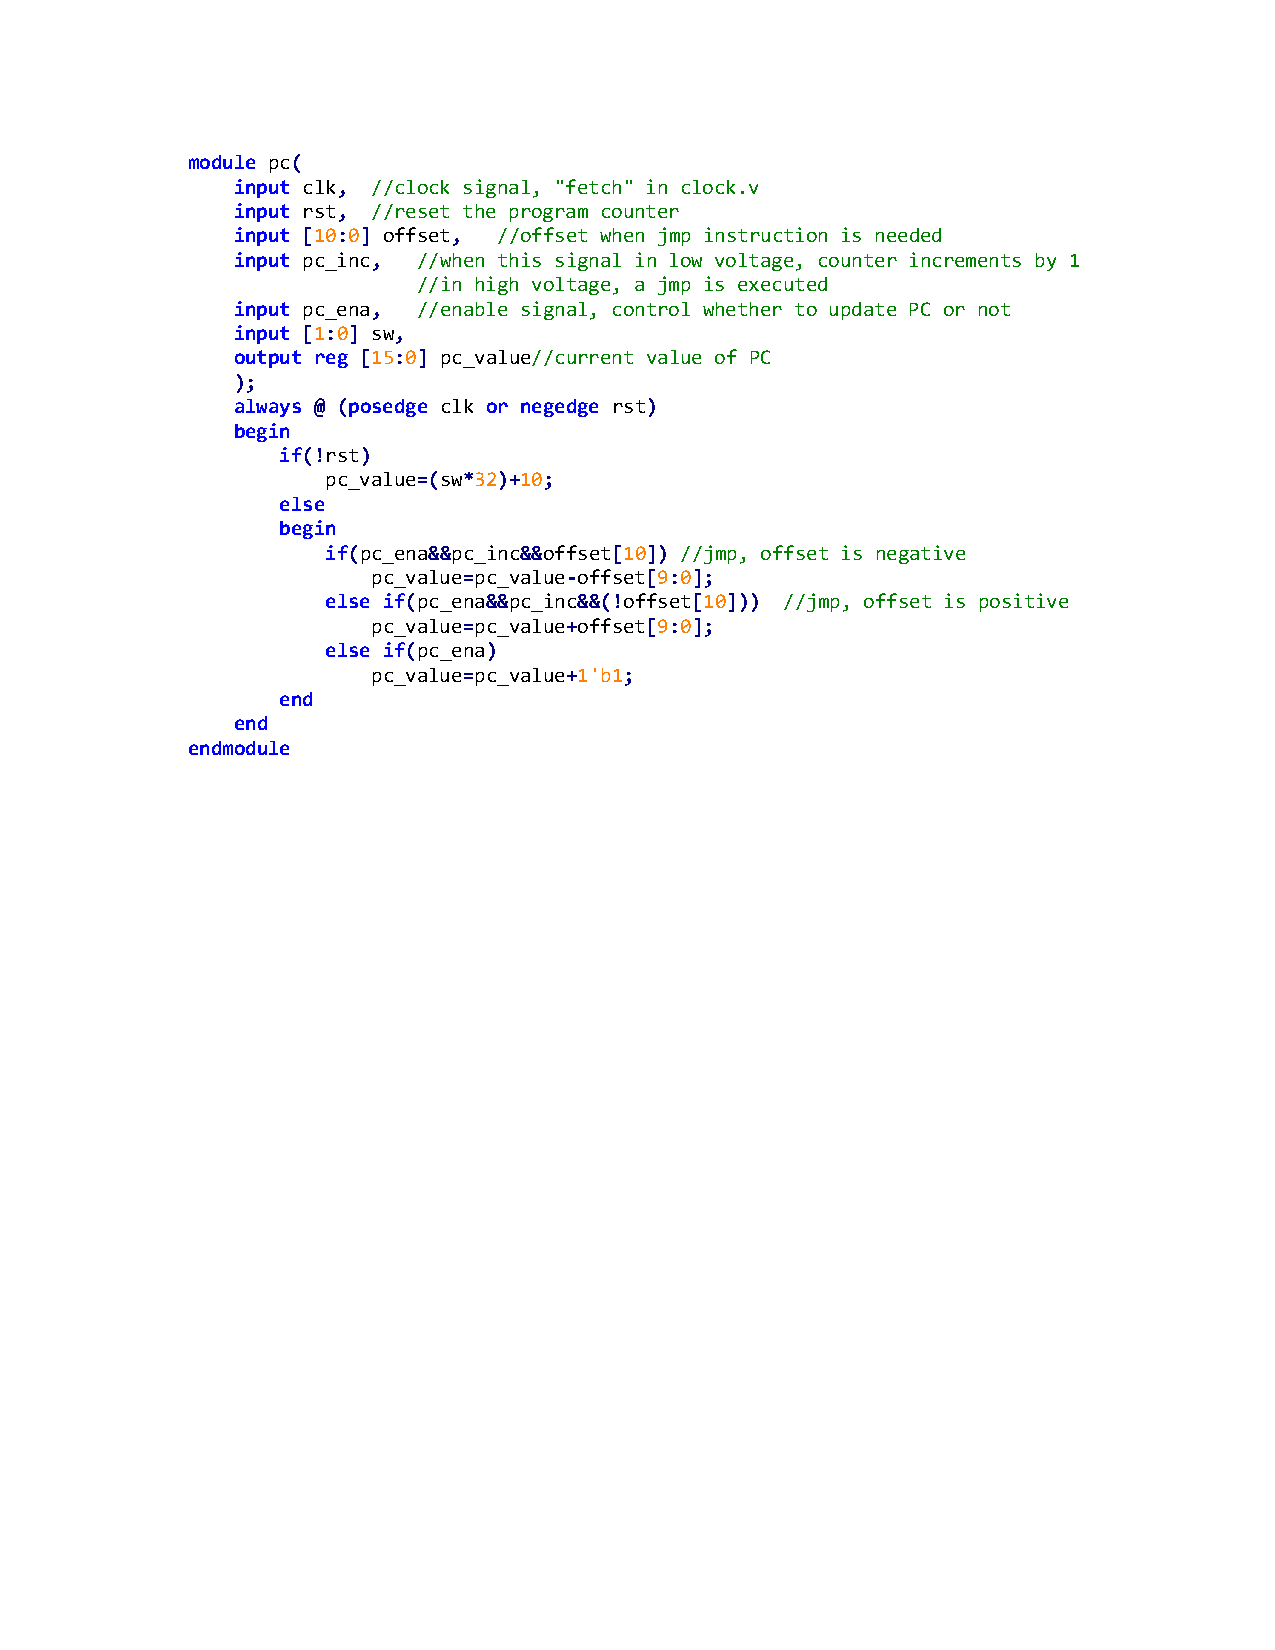
\includegraphics[scale=1]{16.pdf}
			\caption*{代码2: PC模块}
		\end{figure}
		\par 下面是此模块的符号和仿真结果。
		\begin{figure}[H]
			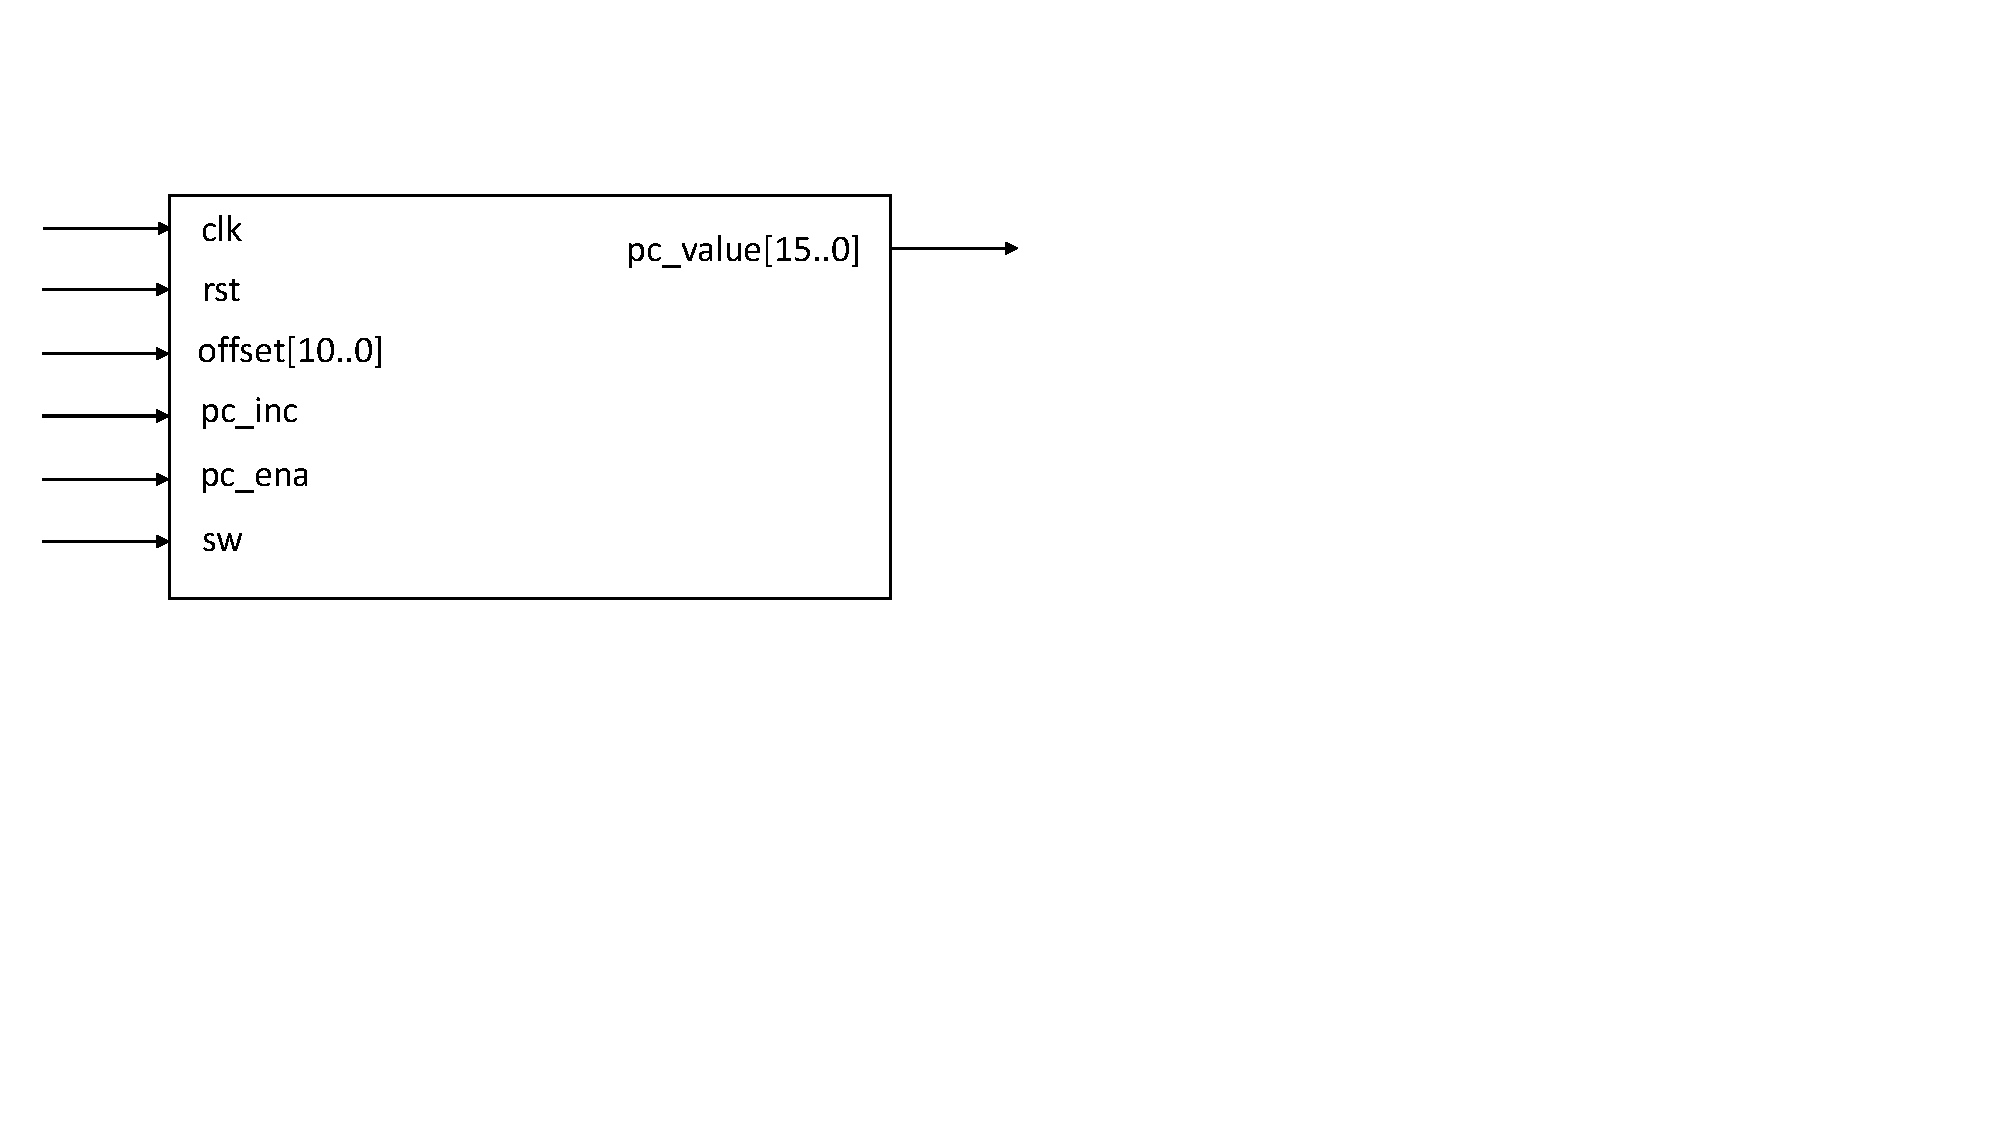
\includegraphics[scale=0.5]{17.pdf}
			\caption{PC模块符号}
		\end{figure}
	\subsection{指令寄存器}
		指令寄存器(Instruction Register, instreg)用于暂存当前正在执行的指令。它的时钟信号是clk,在clk的上升沿触发。指令寄存器将数据总线送来的指令存入16位寄存器中。但总线上传输的数据不需要寄存,因此控制器的ir\_ena信号用来指示数据类型,控制总线数据是否需要寄存。复位(rst置为高位)时,指令寄存器被清零。\par 
		由于每条指令为2个字节,16位,其中高5为为操作码,低11位是偏移地址或目的操作数寄存器和源操作数寄存器,设计中采用的数据总线为16位,每取出一条指令就访存一次。其中,各端口的说明如下:
		\begin{quote}
			输入信号:\\
			$\id{clk}$——时钟信号;\\
			$\id{rst}$——复位信号;\\
			$\id{data}$——数据总线输入;\\
			$\id{ir\_ena}$——IR更新控制。\\
			输出信号:\\
			$\id{ir\_out}$——当前执行的指令,16位二进制串。
		\end{quote}
		\begin{figure}[H]
			\centering
			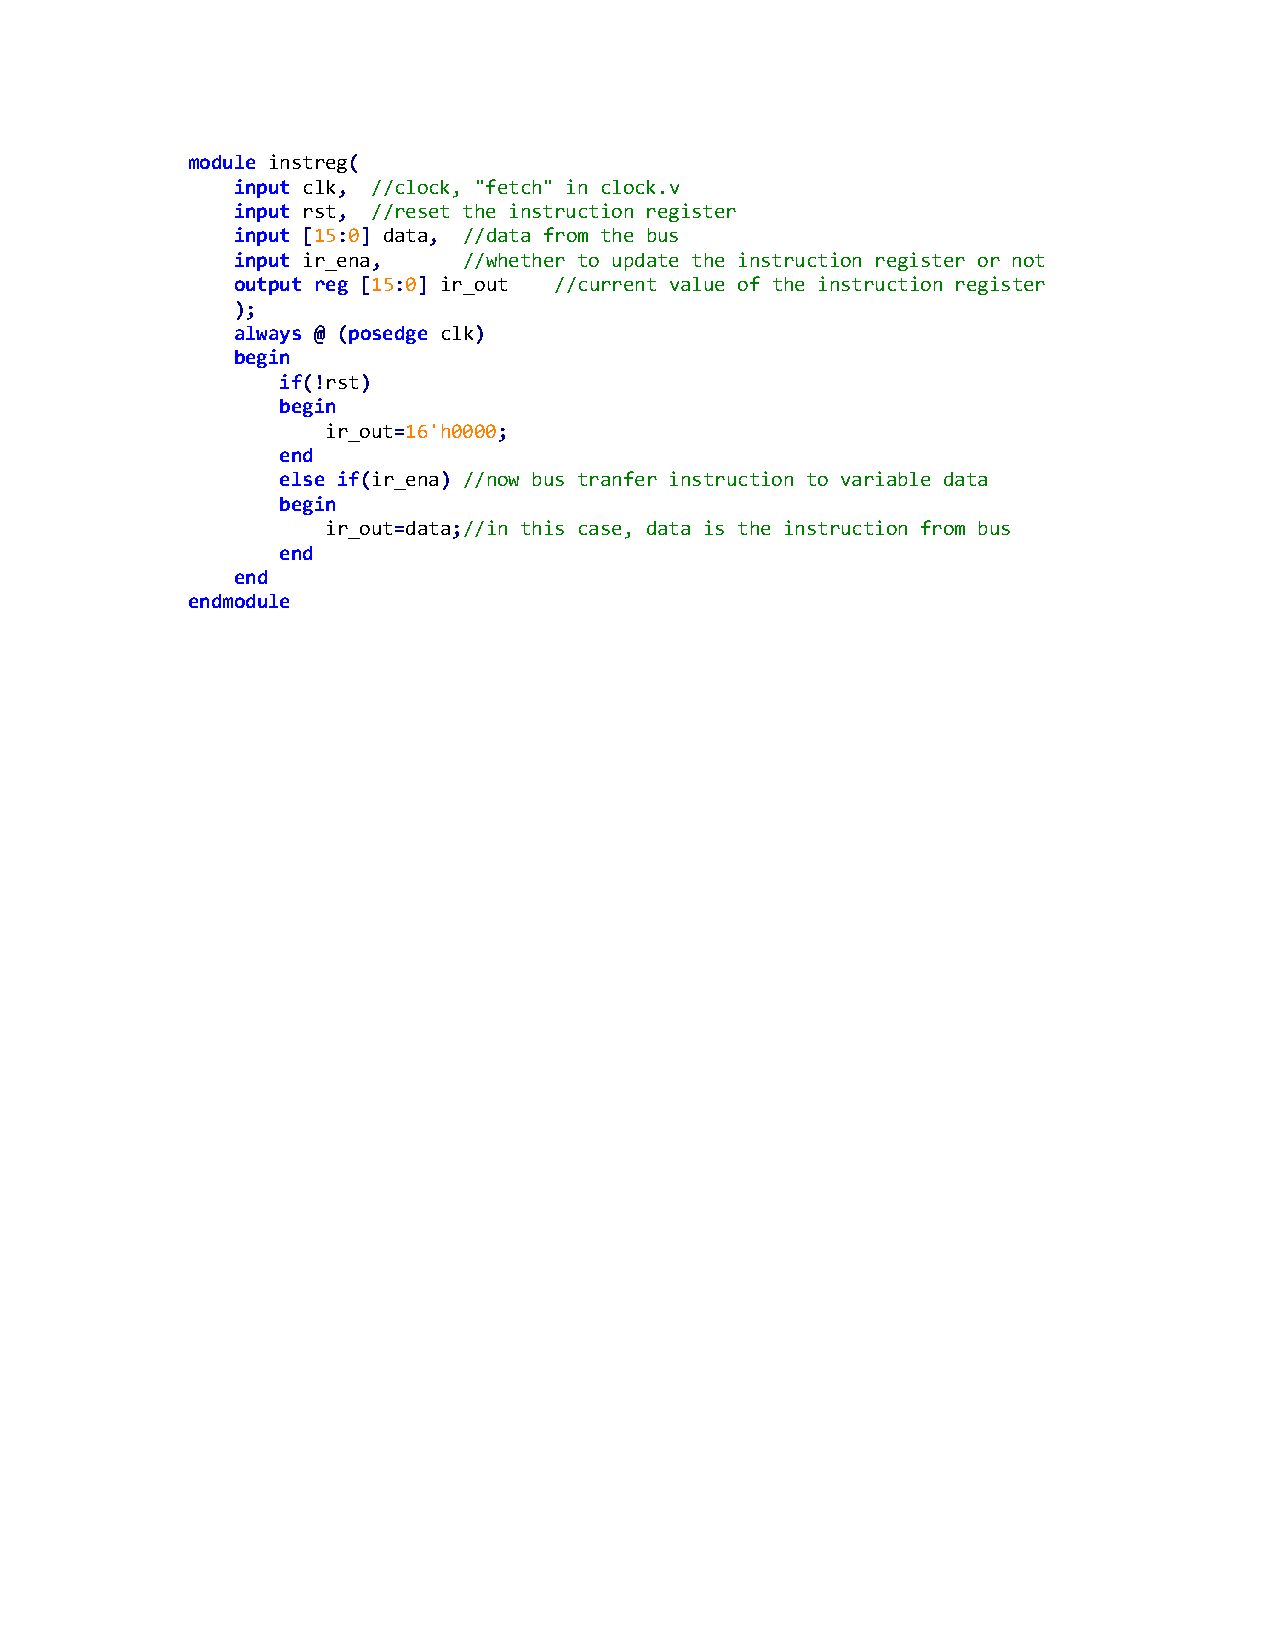
\includegraphics[scale=1]{18.pdf}
			\caption*{代码3: 指令寄存器模块}
		\end{figure}
		\par 下面是此模块的符号和仿真结果。
		\begin{figure}[H]
			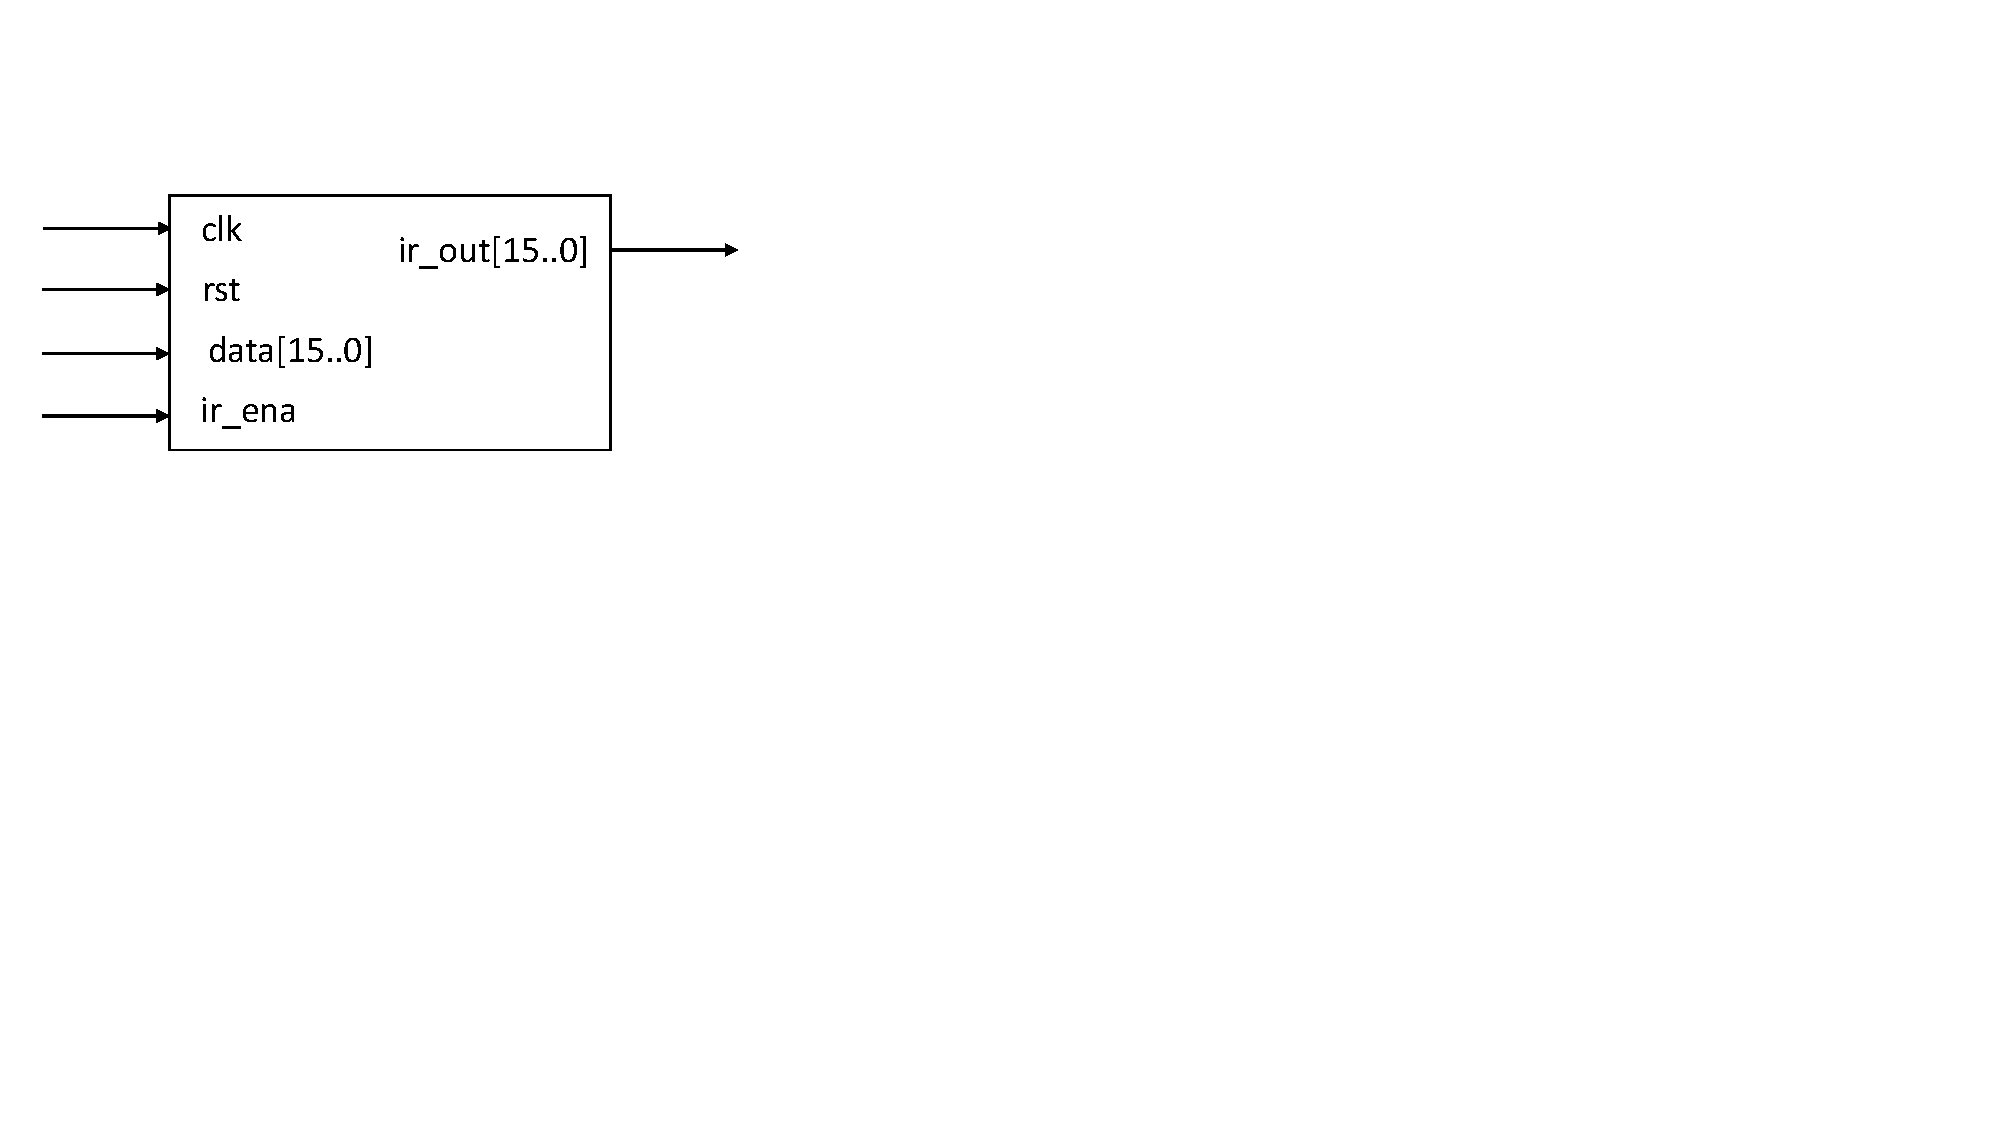
\includegraphics[scale=0.5]{19.pdf}
			\caption*{指令寄存器模块符号}
		\end{figure}
	\subsection{地址寄存器}
	地址寄存器(MAR)是CPU与存储器的一个接口,用于存放待访问的寄存器单元的地址。它的输入和输出关系如下表所示。
		\begin{table}[htb]
		\centering
		\caption{地址寄存器的输入、输出逻辑关系}
		\begin{tabular}{c|c|c|c|c}
			\multicolumn{4}{c|}{输入}         & 输出              \\ \hline
			clk & rst & mar\_ena & mar\_ena & mar\_addr       \\ \hline
			1   & 1   & X        & XX       & 0x0000          \\ \hline
			1   & 0   & 1        & 00       & $\id{pc\_addr}$  \\ \hline
			1   & 0   & 1        & 01       & $\id{ir\_addr1}$ \\ \hline
			1   & 0   & 1        & 10       & $\id{ir\_addr2}$ \\ \hline
			1   & 0   & 1        & 11       & $\id{sp}$       \\ \hline
			0   & X   & X        & X        & 0xXXXX         
		\end{tabular}
	\end{table}\par 
		其各端口信号如下:
		\begin{quote}
		输入信号:\\
		$\id{clk}$——时钟信号;\\
		$\id{rst}$——复位信号;\\
		$\id{mar\_ena}$——MAR输入使能信号;\\
		$\id{mar\_sel}$——MAR输入选择信号,用于选择地址输入;\\
		$\id{ir\_addr1,ir\_addr2}$——来自寄存器的地址;\\
		$\id{pc\_addr}$——PC数据;\\
		$\id{sp\_addr}$——栈指针(SP)数据。\\
		输出信号:\\
		$\id{mar\_addr}$——地址寄存器的输出。
		\end{quote}
		下面是此模块的符号和仿真结果。
		\begin{figure}[H]
			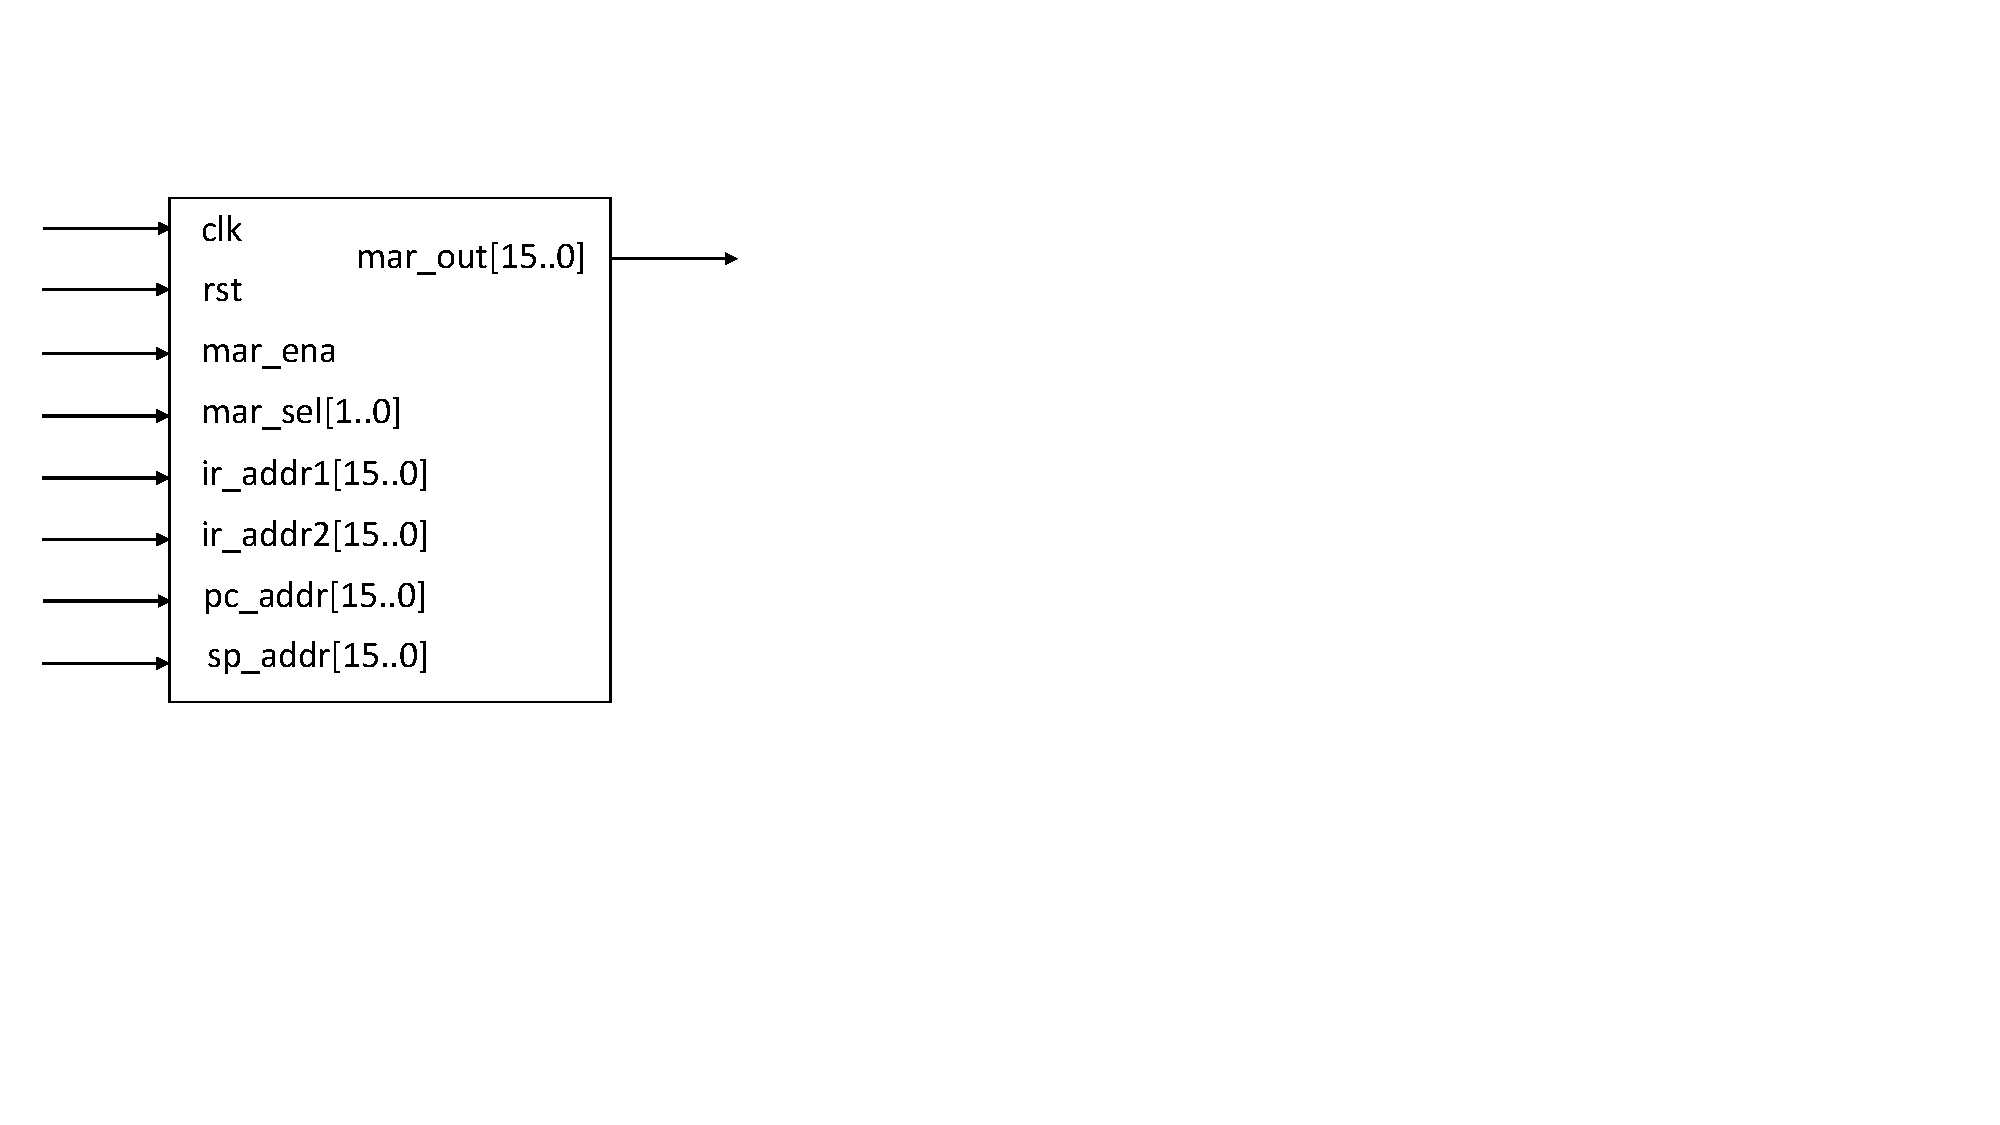
\includegraphics[scale=0.5]{21.pdf}
			\caption{地址寄存器模块的符号}
		\end{figure}
		\begin{figure}[H]
		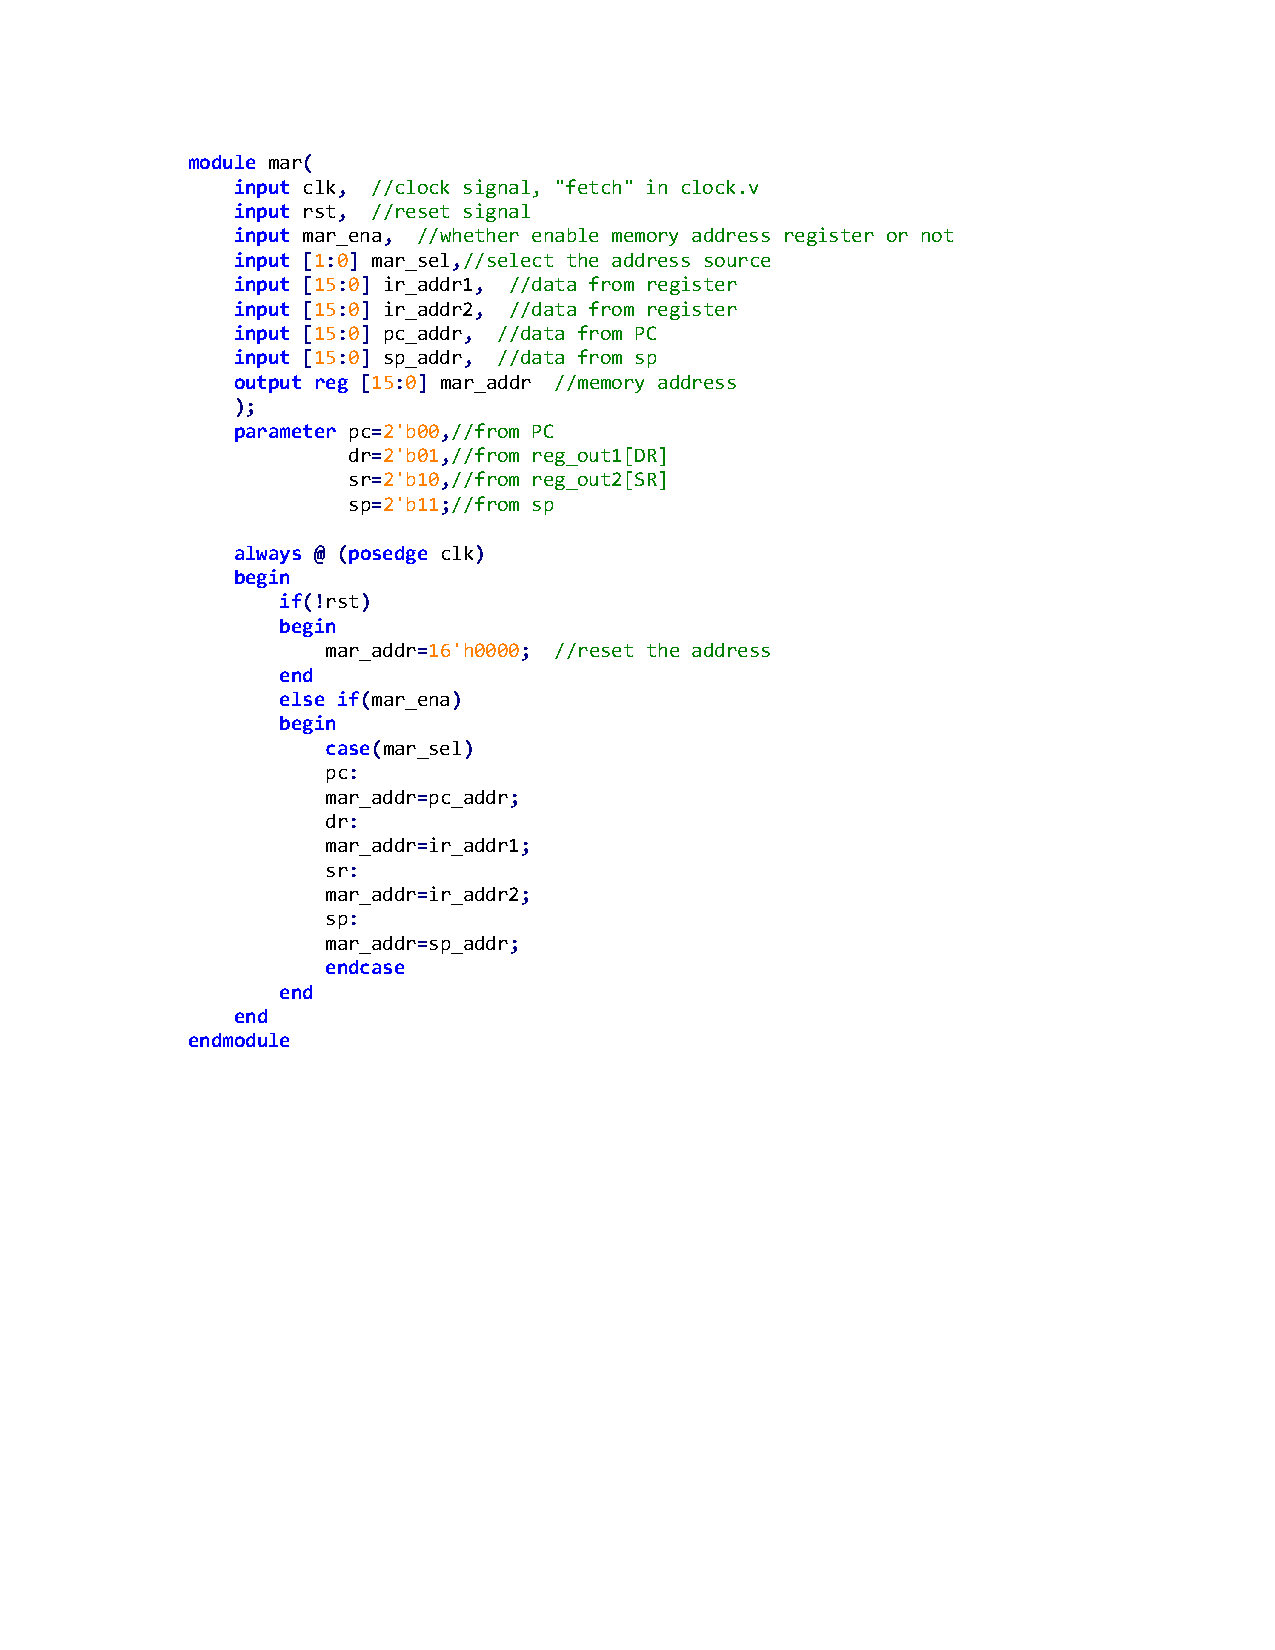
\includegraphics[scale=1]{20.pdf}
		\caption*{代码4: 地址寄存器模块}
		\end{figure}
	\subsection{数据寄存器}
		数据寄存器(MDR)用于将寄存将要被输出到数据总线或送往ALU的数据。各端口的说明如下:
		\begin{quote}
		输入信号:\\
		$\id{clk}$——时钟信号;\\
		$\id{rst}$——复位信号;\\
		$\id{mdr\_ena}$——MDR输入使能信号;\\
		$\id{mdr\_sel}$——MDR输入选择信号,用于选择地址输入;\\
		$\id{reg\_in1,reg\_in2}$——来自寄存器的输入数据;\\
		$\id{mem\_in}$——来自存储器的输入数据。\\
		输出信号:\\
		$\id{mar\_addr}$——向数据总线的数据输出;\\
		$\id{reg\_out}$——向指令寄存器(instreg)的输出。
		\end{quote}
		\begin{table}[htb]
		\centering
		\caption{地址寄存器的输入、输出逻辑关系}
			\begin{tabular}{c|c|c|c|c|c}
			\multicolumn{4}{c|}{输入}         & 输出              \\ \hline
			clk & rst & mdr\_ena & mdr\_ena & mar\_addr&mem\_out       \\ \hline
			1   & 1   & X        & XX       & 0xXXXX&0xXXXX          \\ \hline
			1   & 0   & 1        & 00       & 0xXXXX&0xXXXX  \\ \hline
			1   & 0   & 1        & 01       & $\id{reg\_in1}$&0xXXXX \\ \hline
			1   & 0   & 1        & 10       & $\id{reg\_in2}$&0xXXXX \\ \hline
			1   & 0   & 1        & 11       & 0xXXXX&$\id{mem\_in}$       \\ \hline
			0   & X   & X        & X        & 0xXXXX&0xXXXXX        
			\end{tabular}
		\end{table}
		\begin{figure}[H]
			\centering
			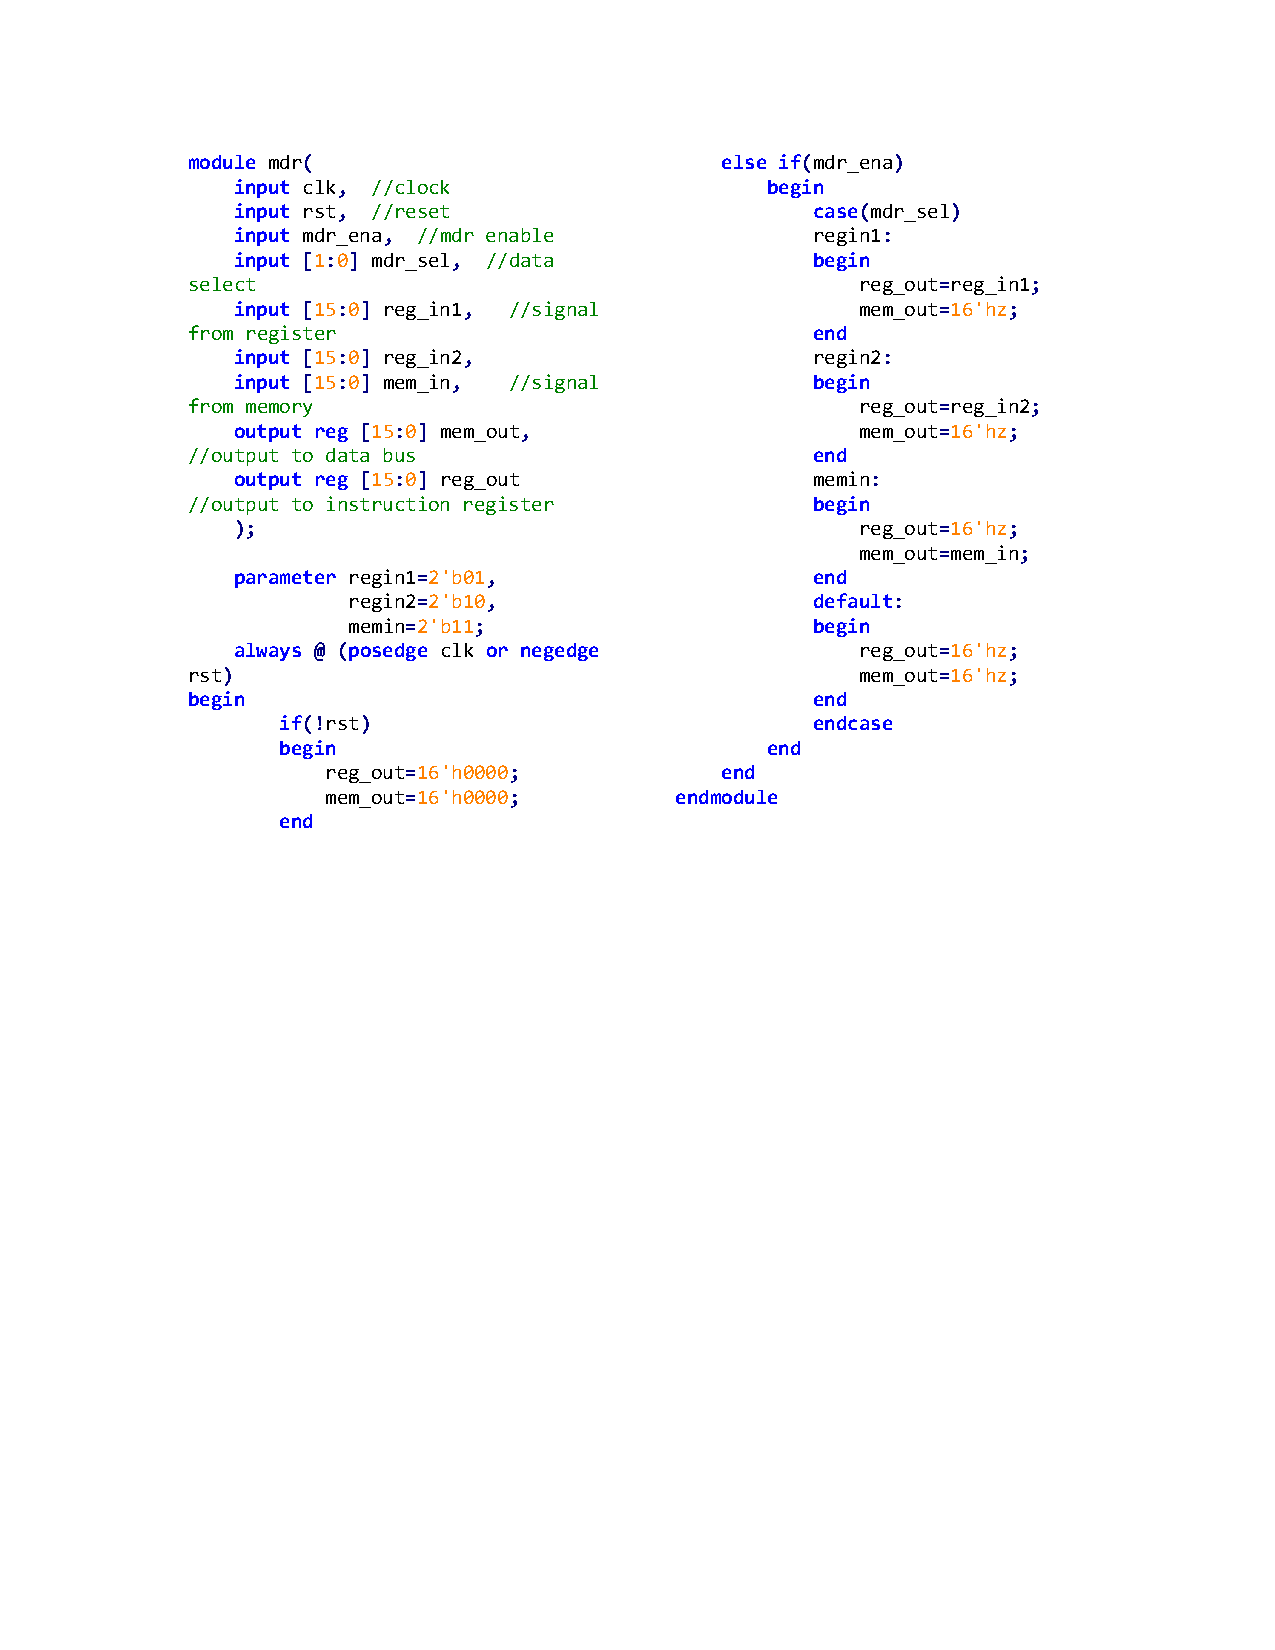
\includegraphics[scale=0.856]{22.pdf}
			\caption*{代码5: 数据寄存器模块}
		\end{figure}
		下面是此模块的符号和仿真结果。
		\begin{figure}[H]
			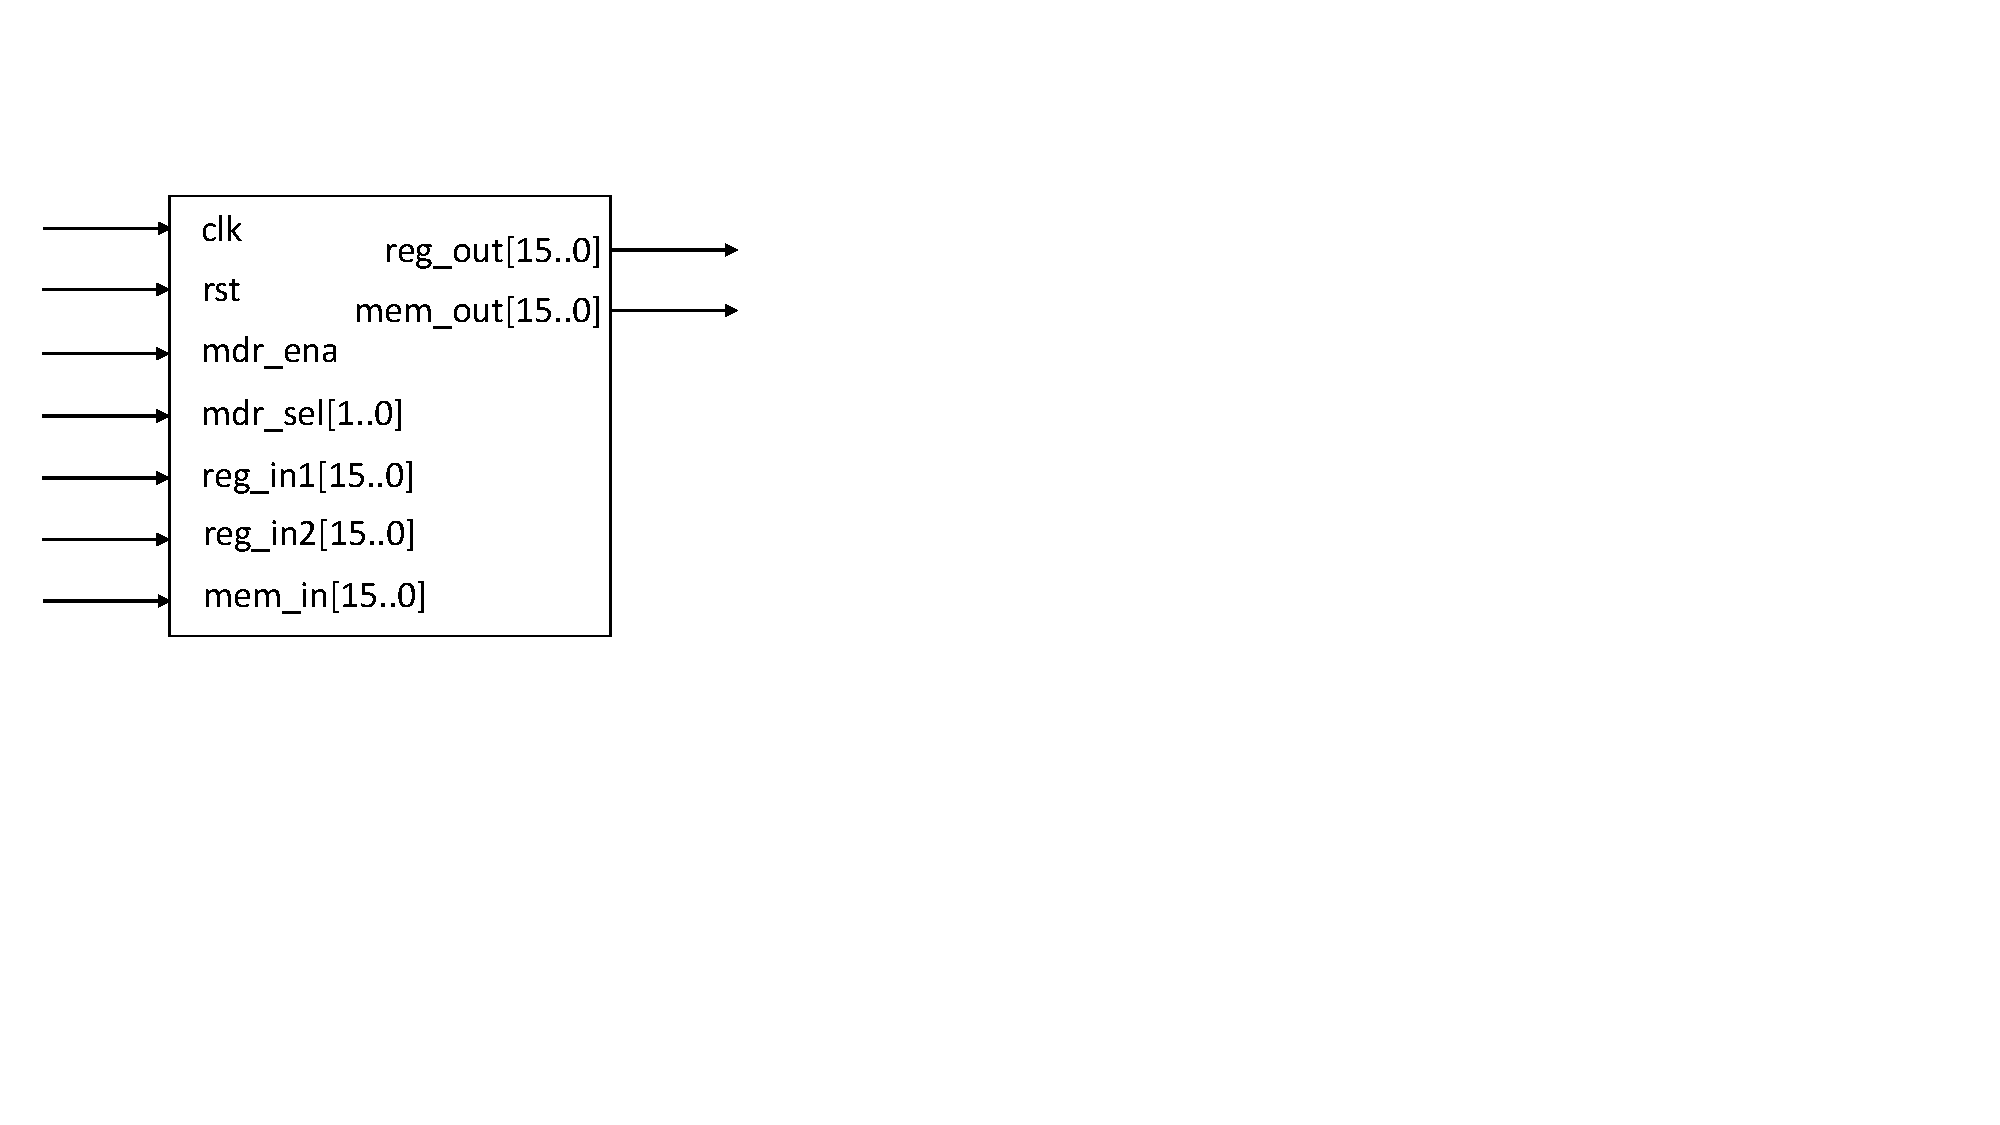
\includegraphics[scale=0.5]{23.pdf}
			\caption*{代码5: 数据寄存器的模块符号}
		\end{figure}
	\subsection{寄存器组}
		寄存器组(Register Array, regarray)用于存储指令执行过程中需要的数据以及指令的执行结果。它一共包含8个16位的通用寄存器,双端口读出、双端口写入,只能按字访问,即一次性读写16位数据。其端口信号说明如下:
		\begin{quote}
			输入信号:\\
			$\id{clk}$——时钟信号;\\
			$\id{rst}$——复位信号;\\
			$\id{reg\_read1}$——端口1读取控制信号(高电平有效);\\
			$\id{reg\_read2}$——端口2读取控制信号(高电平有效);\\
			$\id{addr1}$——端口1地址信号;\\
			$\id{addr2}$——端口2地址信号;\\
			$\id{reg\_write1}$——端口1写入控制信号(高电平有效);\\
			$\id{reg\_write2}$——端口2写入控制信号(高电平有效);\\
			$\id{data\_in1,data\_in2,data\_in3}$——3个输入信号。\\
			输出信号:\\
			$\id{reg\_out1}$——读端口1输出数据;\\
			$\id{reg\_out2}$——读端口2输出数据。	
		\end{quote}\par 
		寄存器组的3路16位输入数据分别为data\_in1, data\_in2, data\_in3。2路16位读出数据分别为reg\_out1, reg\_out2。2个端口的读取控制信号分别为reg\_read1, reg\_read2,写入控制信号分别为reg\_write1, reg\_write2。从寄存器组读出的数据可以送到ALU的数据输入端的多路选择器,也可以是访存指令地址。数据寄存器原理上只能按字节读写,但是为了支持涉及到8位数据的操作指令\footnote{MOVIL \$IMM, \%DR,MOVIH \$IMM, \%DR,具体功能见第\hyperpage{4}页表格。},使用以下方法来支持它们。当进行8位数据的写操作时:
		\begin{enumerate}
			\item 读数据阶段:将目的寄存器(DR)的数据取出;
			\item 指令执行阶段:将指令中的8位立即数(IMM)拼接到目的寄存器(DR)的相应1字节的位置上;
			\item 回写阶段:将拼接后的结果写回目的寄存器(DR)中。
		\end{enumerate}
		\par 这样的设计可以简化寄存器组的读写控制逻辑,实现代码如下:
		\begin{figure}[H]
			\centering
			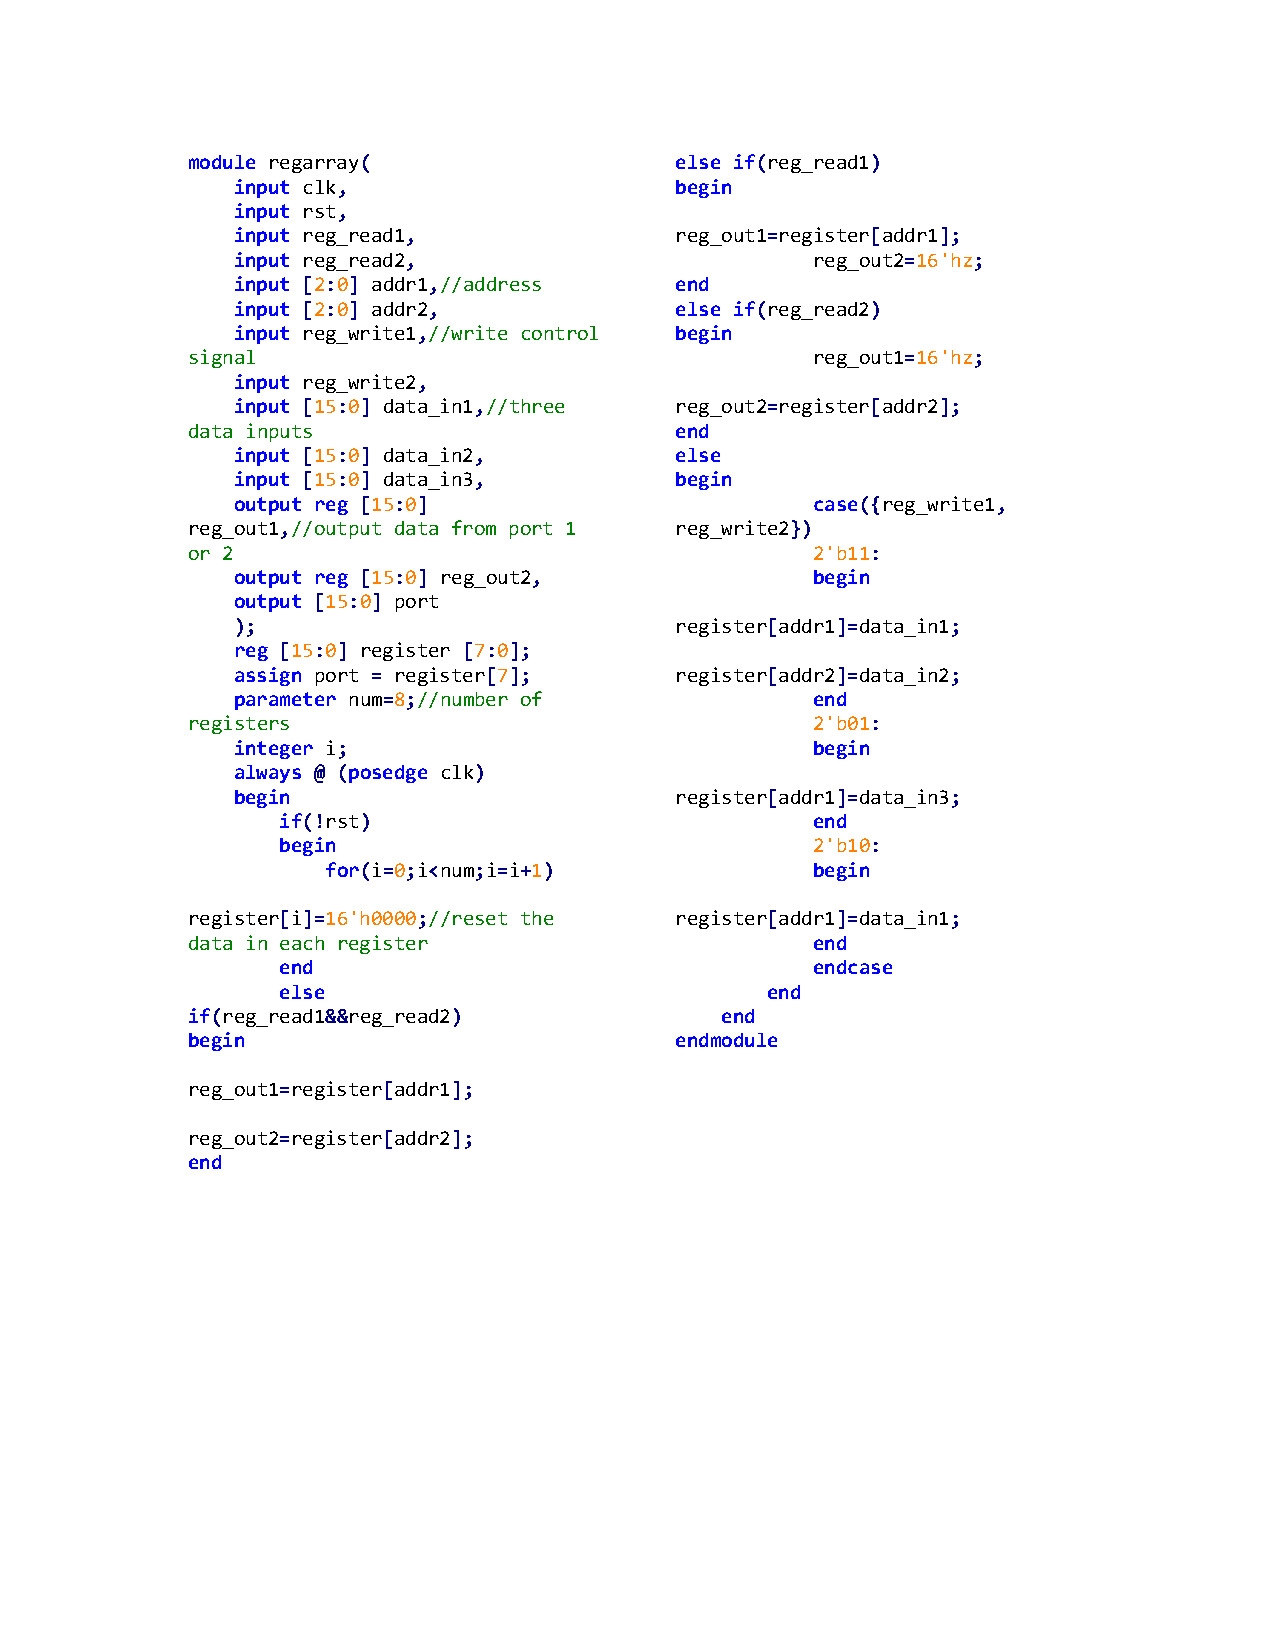
\includegraphics[scale=0.961]{24.pdf}
			\caption*{代码6: 寄存器组模块}
		\end{figure}
		此模块的符号如下:
		\begin{figure}[H]
			\centering
			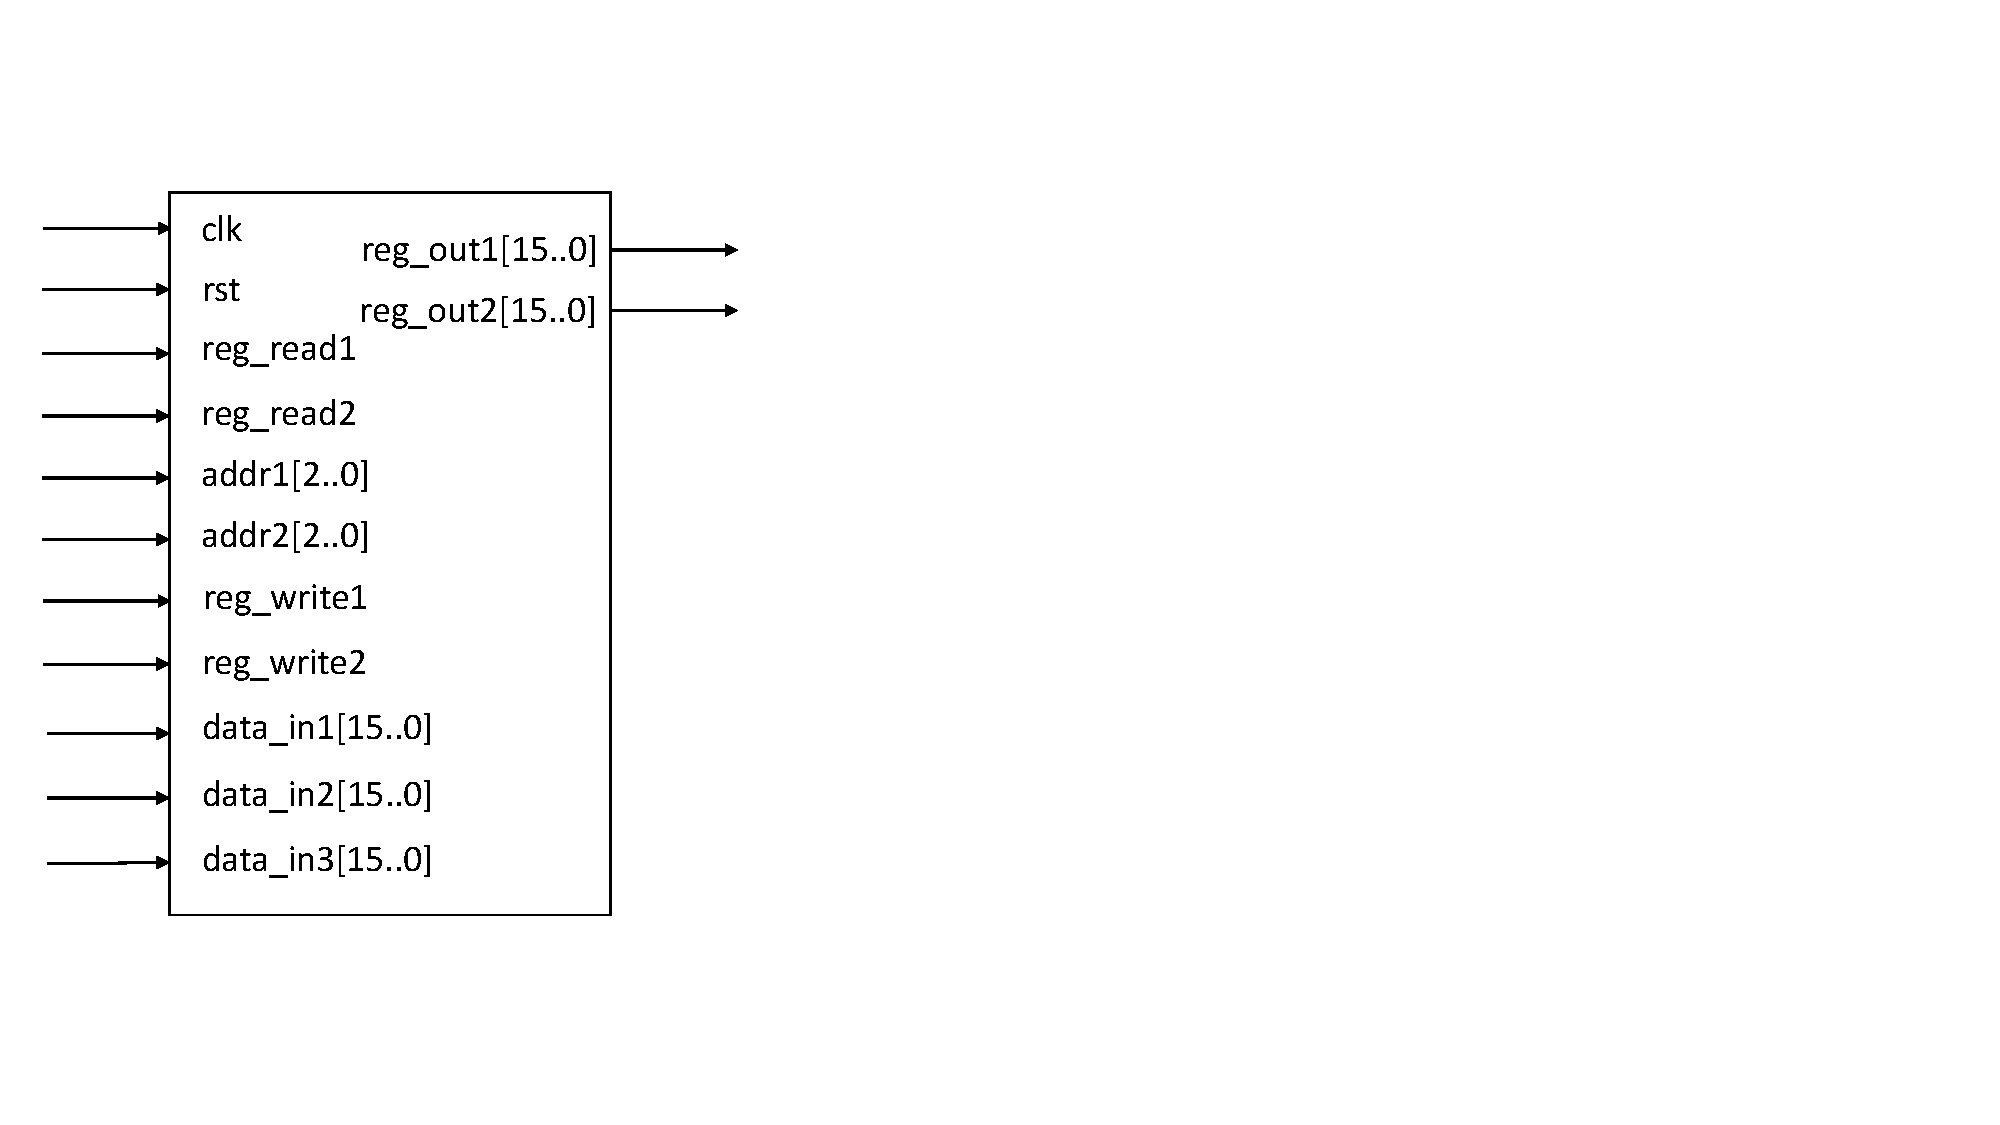
\includegraphics[scale=0.5]{25.pdf}
			\caption{寄存器组的模块符号}
		\end{figure}
	\subsection{栈指针寄存器}
		栈指针寄存器(SP)是用于存储栈顶地址的。入栈(PUSH)和出栈(POP)指令访问的存储单元是由SP发出的。我们规定CPU栈顶起始地址为0x0200,也即初始化时SP的值。当执行入栈指令(PUSH)时,控制信号sp\_push有效,SP自增1;执行出栈(POP)指令时,控制信号sp\_pop有效,SP自减1。其各端口信号说明如下:
			\begin{quote}
				输入信号:\\
				$\id{clk}$——时钟信号;\\
				$\id{rst}$——复位信号;\\
				$\id{sp\_push}$——入栈控制信号;\\
				$\id{sp\_pop}$——出栈控制信号。\\
				输出信号:\\
				$\id{sp\_value}$——栈顶地址。
			\end{quote}
			\begin{figure}[H]
				\centering
				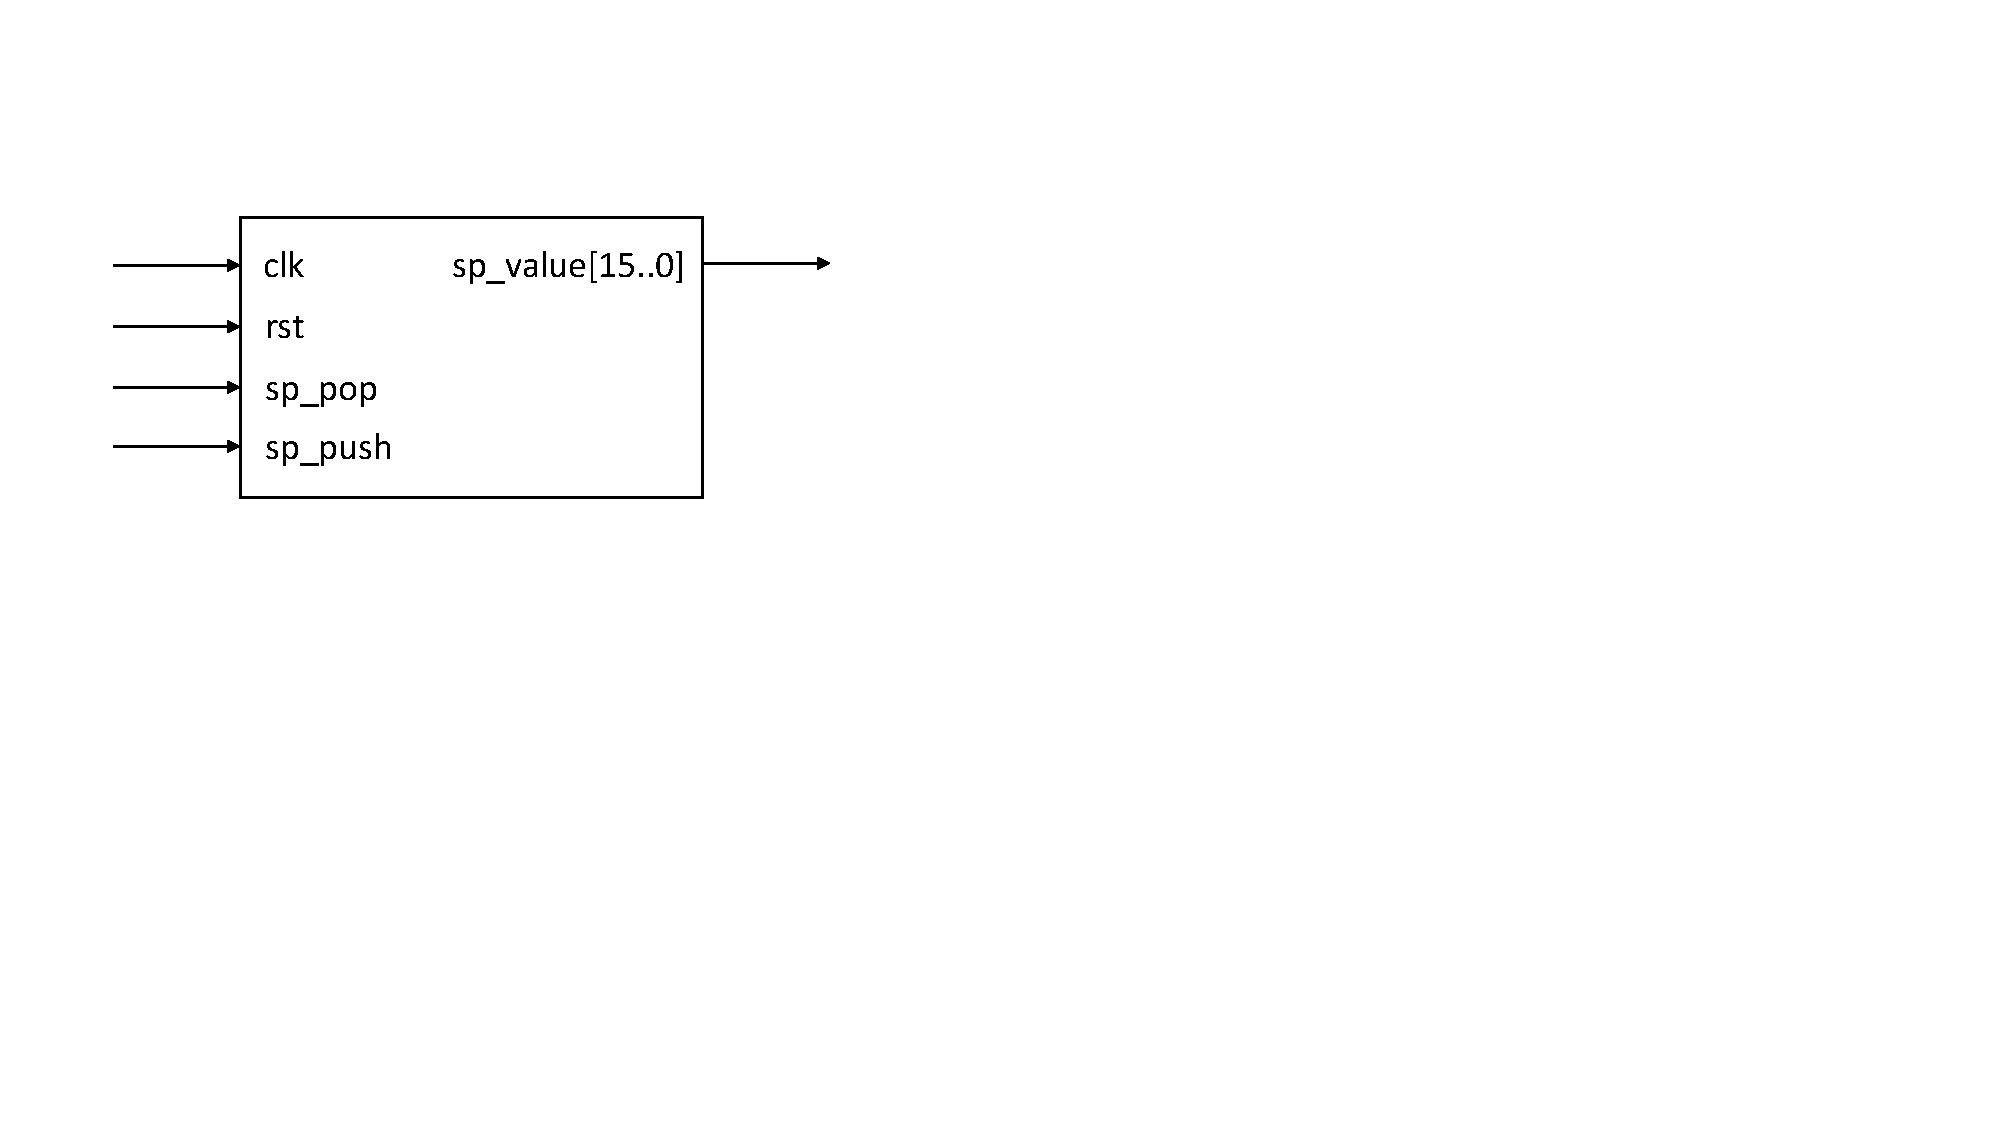
\includegraphics[scale=0.5]{27.pdf}
				\caption{栈指针寄存器的模块符号}
			\end{figure}
			\begin{figure}[H]
				\centering
				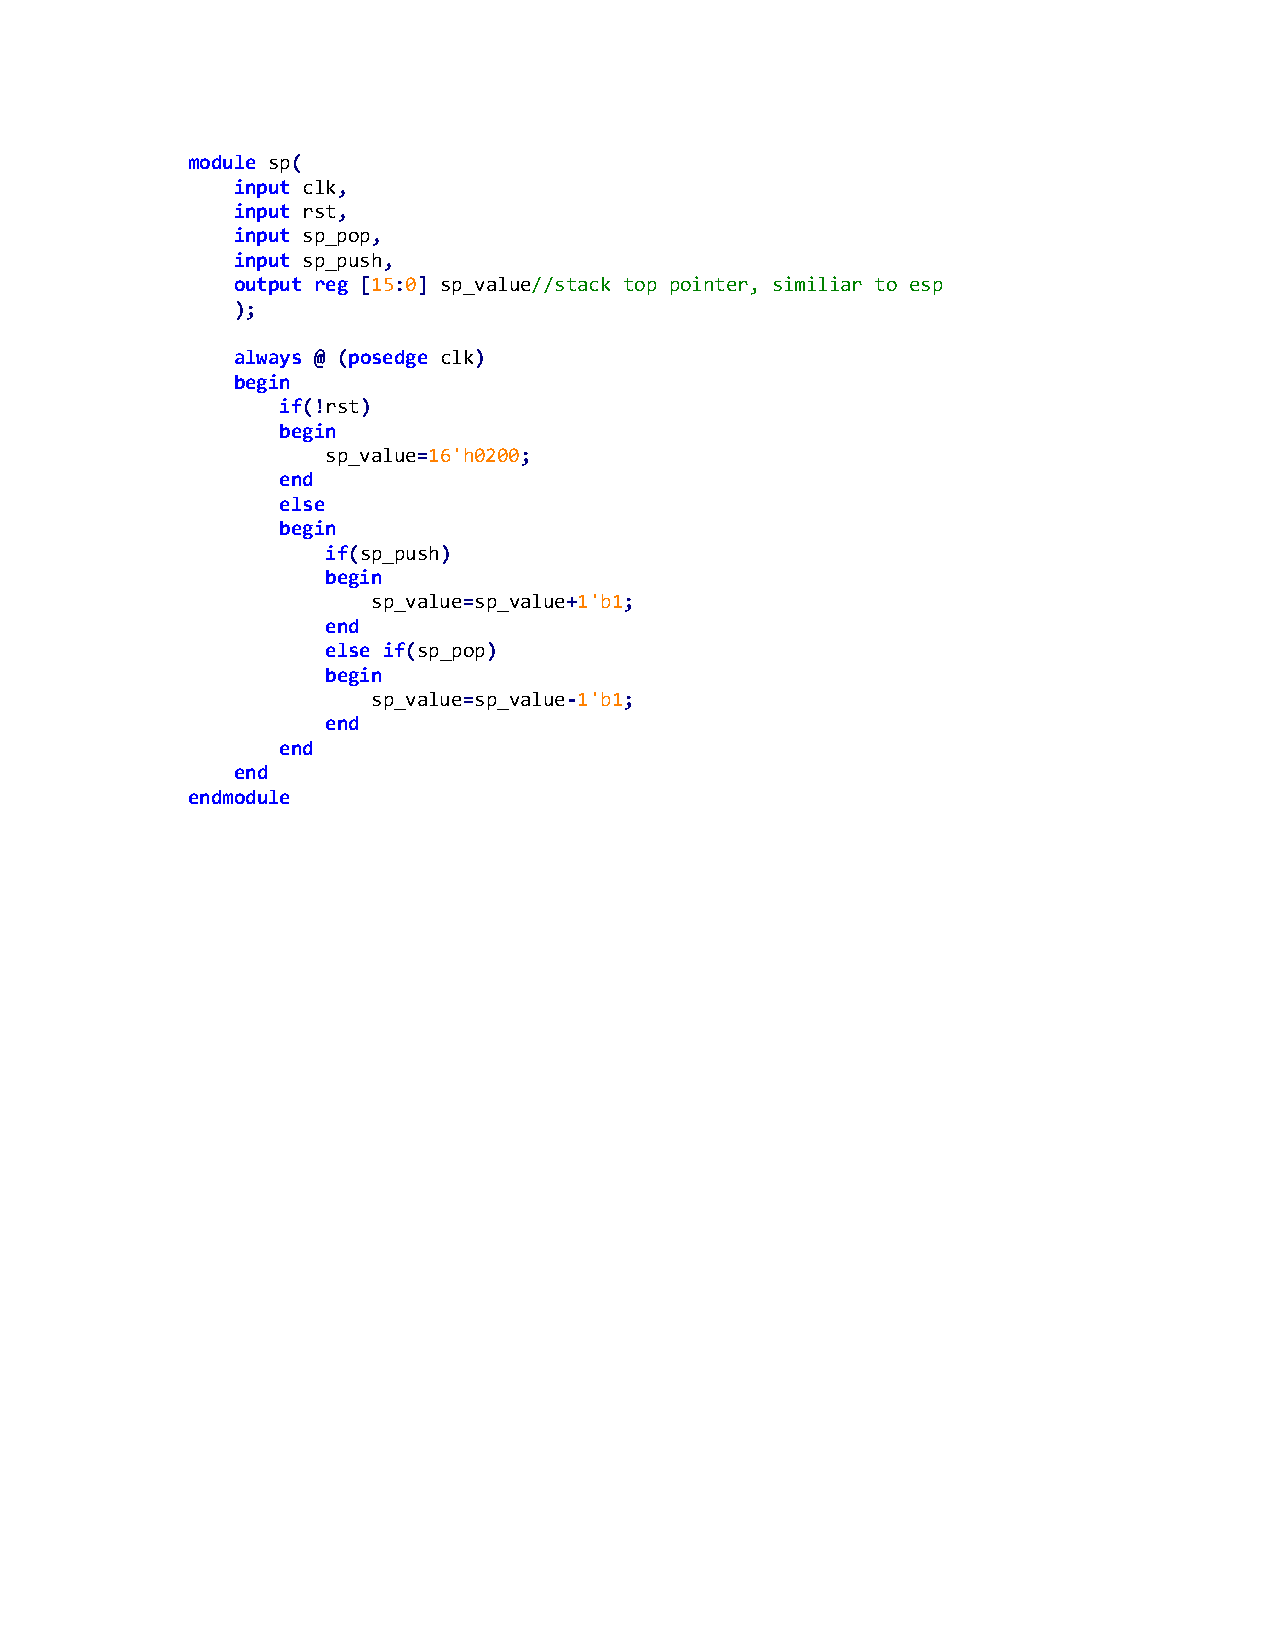
\includegraphics[scale=1]{26.pdf}
				\caption*{代码7: 栈指针寄存器模块}
			\end{figure}
			
\end{document}